\subsection{Finding a stable matching}
\label{sec:threed_sr_as_findingastablematching}

\subsubsection{Preliminaries}

In this section we show that every such instance of 3DR-AS contains a stable matching, which can be found in $O(|N|^3)$ time. We give a step-by-step constructive proof of this result between Sections~\ref{sec:threed_sr_as_removingtriangles}--\ref{sec:threed_sr_as_symmetric_binary_finding_in_general}.

For technical purposes, in this section (Section~\ref{sec:threed_sr_as_findingastablematching}) only, we make two relaxations to the model described in Section~\ref{sec:threed_sr_as_model}. In fact, we prove a slightly more general result than required. Firstly, we suppose an instance $(N, V)$ of 3DR-AS may contain a number of agents that is not necessarily divisible by three. Secondly, we define a \emph{matching} only as a set of triples, which does not necessarily partition $N$. For any matching $M$ and any agent $\alpha_i$, if no triple in $M$ contains $\alpha_i$ then we say that $\alpha_i$ is \emph{unmatched} in $M$ and write $M(\alpha_i) = \varnothing$. All other definitions and notation remain the same. Thus, in this section we show that any (relaxed) instance of 3DR-AS contains a (relaxed) stable matching. Now, for any (relaxed) instance of 3DR-AS and (relaxed) stable matching $M$, if the number of agents is divisible by three (and thus the instance meets the original definition) then any unmatched agents may be arbitrarily matched into triples. It follows by Proposition~\ref{prop:threed_sr_as_blockerimprovement} that the resulting (non-relaxed) matching $M'$ is stable in the (non-relaxed) instance, as required.

We also introduce a restricted type of (relaxed) matching called a \emph{$P$\nobreakdash-matching}. Recall that by definition, $M(\alpha_p)=\varnothing$ implies that $u_{\alpha_p}(M)=0$ for any $\alpha_p \in N$ in an arbitrary (relaxed) matching $M$. We say that a matching $M$ in $(N, V)$ is a \emph{$P$\nobreakdash-matching} if $M(\alpha_p) \neq \varnothing$ implies $u_{\alpha_p}(M) > 0$. A $P$\nobreakdash-matching thus corresponds to a $\{ K_3, P_3 \}$-packing in the underlying graph \cite{KH83}. Note that any triple in a $P$\nobreakdash-matching $M$ must contain at least one agent with utility two. A \emph{stable $P$\nobreakdash-matching} is a $P$\nobreakdash-matching that is also stable. Our main result is that any instance of 3DR-AS with binary and symmetric preferences contains a stable $P$\nobreakdash-matching.

\subsubsection{Removing triangles}
\label{sec:threed_sr_as_removingtriangles}

In an instance $(N, V)$ of 3DR-AS with binary and symmetric preferences, a \emph{triangle} comprises three agents $\alpha_{m_1}, \alpha_{m_2},\allowbreak \alpha_{m_3}$ such that $v_{\alpha_{m_1}}(\alpha_{m_2}) = v_{\alpha_{m_2}}(\alpha_{m_3}) = v_{\alpha_{m_3}}(\alpha_{m_1}) = 1$. If $(N, V)$ contains no triangle then we say it is \emph{triangle-free}. If $(N, V)$ is not triangle-free then it can be reduced, by successively removing triangles, until it is triangle-free. This operation is our first step towards constructing a stable $P$\nobreakdash-matching in $(N, V)$. We formalise this result in Lemma~\ref{lem:threed_sr_as_symmetric_binary_trianglefree}.

\begin{lem}
\label{lem:threed_sr_as_symmetric_binary_trianglefree}
Given an instance $(N, V)$ of 3DR-AS with binary and symmetric preferences, we can, in $O(|N|^3)$ time, identify an instance $(N', V')$ of 3DR-AS with binary and symmetric preferences and a $P$\nobreakdash-matching $M_{\triangle}$ such that $(N', V')$ is triangle-free, $|N'|\leq |N|$, and if $M$ is a stable $P$\nobreakdash-matching in $(N', V')$ then $M' = M \cup M_{\triangle}$ is a stable $P$\nobreakdash-matching in $(N, V)$.
\end{lem}
\begin{proof}
Construct $M_{\triangle}$ as a \emph{maximal triangle packing} \cite{CHATAIGNER20091396} in the underlying graph, in $O(|N|^3)$ time. Let $N' = N \setminus \bigcup M_{\triangle}$. Construct $V'$ accordingly. By definition, $M_{\triangle}$ is a $P$\nobreakdash-matching, $(N', V')$ is triangle-free, and $|N'| \leq |N|$. 

Suppose $M$ is a stable $P$\nobreakdash-matching in $(N', V')$. Consider $M' = M \cup M_{\triangle}$. By definition, $M'$ is a $P$\nobreakdash-matching. Since each triple in $M_{\triangle}$ corresponds to a triangle, any agent in any triple in $M_{\triangle}$ must have utility two in $M_{\triangle}$ and thus does not belong to a triple that blocks $M'$ in $(N, V)$. If some triple blocks $M'$ in $(N, V)$ then it must contain three agents in $N'$, and thus it must also block $M$ in $(N', V')$, which is impossible. It follows that $M'$ is stable in $(N, V)$.
\end{proof}

\subsubsection{Repairing a \texorpdfstring{$P$}{P}-matching in a triangle-free instance}
\label{sec:threed_sr_as_symmetric_binary_repairing}

In this section (Section~\ref{sec:threed_sr_as_symmetric_binary_repairing}), we consider instances of 3DR-AS that are triangle-free, and in them define a special type of $P$\nobreakdash-matching that is \emph{repairable}. 

We present Subroutine~\algorithmfont{repair}, shown in Algorithms~\ref{alg:threed_sr_as_almostthere_algo_phase1} and~\ref{alg:threed_sr_as_almostthere_algo_phase2} which, given a triangle-free instance $(N, V)$ and a repairable $P$\nobreakdash-matching $M$, constructs a new $P$\nobreakdash-matching $M'$ that is stable in $(N, V)$. We shall see in the next section (Section~\ref{sec:threed_sr_as_symmetric_binary_finding_in_triangle_free}) how this subroutine is used in a more general subroutine that, given a triangle-free instance of 3DR-AS, returns a $P$\nobreakdash-matching that is stable.

Given a triangle-free instance $(N, V)$ and a $P$\nobreakdash-matching $M$, we say that $M$ is \emph{repairable} if it is not stable and there exists some $\alpha_i \in N$ such that $u_{\alpha_i}(M)=0$ and any triple that blocks $M$ comprises $\{ \alpha_i, \alpha_{j_1}, \alpha_{j_2}\}$ for some $\alpha_{j_1}, \alpha_{j_2}\in N$ where $u_{\alpha_{j_1}}(M)=1$, $u_{\alpha_{j_2}}(M)=0$, and $v_{\alpha_i}(\alpha_{j_1})=v_{\alpha_{j_1}}(\alpha_{j_2})=1$.

We now provide some intuition behind Subroutine~\algorithmfont{repair} and refer the reader to Figure~\ref{fig:threed_sr_as_symmetric_binary_repair_algorithm_7_cases_original_case}. Recall that the overall goal of the subroutine is to construct a $P$\nobreakdash-matching $M'$ that is stable. Since $M$ is repairable, our goal will be to modify $M$ in such a way that $u_{\alpha_i}(M')\geq 1$ and no triple blocks $M'$ that did not also block $M$. By the definition of repairable, and Proposition~\ref{prop:threed_sr_as_blockerimprovement}, it follows that the resulting $P$\nobreakdash-matching $M'$ is stable. For example, one way to accomplish this goal would be to construct $M'$ in such a way that $u_{\alpha_i}(M')\geq 1$ and $u_{\alpha_p}(M')\geq u_{\alpha_p}(M)$ for any $\alpha_p \in N\setminus \{ \alpha_i \}$, from which it would follow by Proposition~\ref{prop:threed_sr_as_blockerimprovement} that $M'$ is stable.

\begin{figure}
    \centering
    
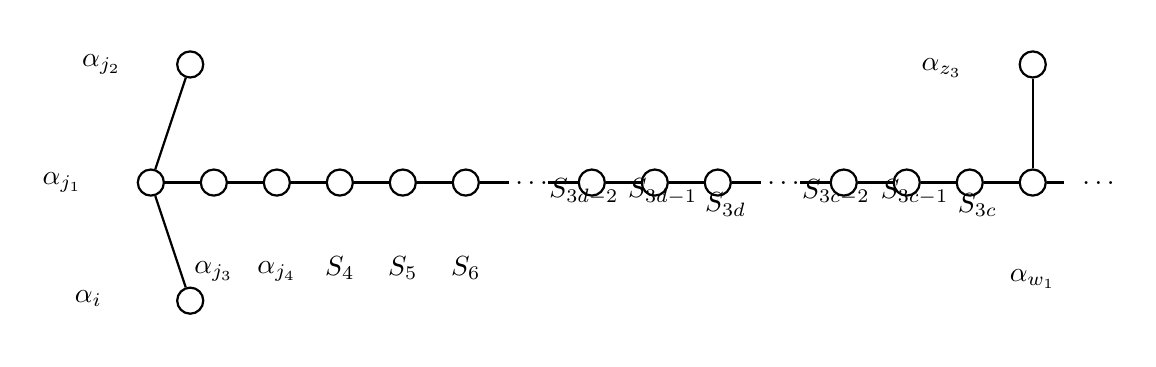
\begin{tikzpicture}
\centering
\begin{scope}[every node/.style={circle,draw, minimum size=2.4mm}, xscale=1.0]
    \node[thick, circle, label={[label distance=0.5cm]180:$\alpha_{i\phantom{j_2}}$}] (ai) at (1,0.5) {};
    \node[thick, circle, label={[label distance=0.5cm]180:$\alpha_{j_2}$}] (aj2) at (1,3.5) {};
    \node[thick, circle, label={[label distance=0.5cm]180:$\alpha_{j_1}$}] (aj1) at (0.5,2) {};
    \node[thick, circle, label={[label distance=0.5cm]270:$\alpha_{j_3}$}] (aj3) at (1.3,2) {};
    \node[thick, circle, label={[label distance=0.5cm]270:$\alpha_{j_4}$}] (aj4) at (2.1,2) {};
    
    \node[thick, circle, label={[label distance=0.5cm]270:$S_{4}$}] (s4) at (2.9,2) {};
    \node[thick, circle, label={[label distance=0.5cm]270:$S_{5}$}] (s5) at (3.7,2) {};
    \node[thick, circle, label={[label distance=0.5cm]270:$S_{6}$}] (s6) at (4.5,2) {};
    
    \node[fill=white, rectangle, draw=white, text =black, minimum size=0, inner sep=0] (dots1) at (5.3,2) {\hspace{2pt}$\dots$};
    
    % \node[circle, minimum size=1mm, inner sep = 0, blue] (abc) at (5.3, 2) {};
    
    \node[thick, circle, label={[shift={(-0.1, -0.925)}]:$S_{3d-2}$}] (s3d2) at (6.1,2) {};
    \node[thick, circle, label={[shift={(0.1, -0.925)}]:$S_{3d-1}$}] (s3d1) at (6.9,2) {};
    \node[thick, circle, label={[shift={(0.1, -0.925)}]:$S_{3d}$}] (s3d) at (7.7,2) {};
    
    \node[fill=white, rectangle, draw=white, text =black, minimum size=0, inner sep=0] (dots2) at (8.5,2) {\hspace{2pt}$\dots$};
    
    \node[thick, circle, label={[shift={(-0.1, -0.925)}]:$S_{3c-2}$}] (s3c2) at (9.3,2) {};
    \node[thick, circle, label={[shift={(0.1, -0.925)}]:$S_{3c-1}$}] (s3c1) at (10.1,2) {};
    \node[thick, circle, label={[shift={(0.1, -0.925)}]:$S_{3c}$}] (s3c) at (10.9,2) {};
    
    \node[thick, circle, label={[label distance=0.5cm]270:$\alpha_{w_1}\vphantom{S_{3d-1}}$}] (aw1) at (11.7,2) {};
    \node[rectangle, white, text=black, fill=white, minimum width=8mm, minimum height=12mm, inner sep=0.5mm] (aw2) at (12.5,2) {\hspace{2pt}$\dots$};
    
    \node[thick, circle, label={[label distance=0.5cm]180:$\alpha_{z_3}\vphantom{S_{3d-1}}$}] (az3) at (11.7,3.5) {};
    
    \dashedcontainerthing{aj2};
    \dashedcontainerthing{ai};
    \dashedcontainerthing{aj1,aj3,aj4};
    \dashedcontainerthing{s4,s5,s6};
    \dashedcontainerthing{s3d2,s3d1,s3d};
    \dashedcontainerthing{s3c2,s3c1,s3c};
    \dashedcontainerthing{aw1,aw2};
    \dashedcontainerthing{az3};
\end{scope}
\begin{scope}
    \foreach \from/\to in {aj2/aj1, aj1/ai, aj1/aj3, aj3/aj4, aj4/s4, s4/s5, s5/s6, s6/dots1, dots1/s3d2, s3d2/s3d1, s3d1/s3d, s3d/dots2, dots2/s3c2, s3c2/s3c1, s3c1/s3c, s3c/aw1, aw1/az3, aw1/aw2}
        \draw [thick] (\from) -- (\to);
\end{scope}

\end{tikzpicture}
    \caption[Agents and triples in $M$ before a new iteration of the while loop]{Agents and triples in $M$ before a new iteration of the while loop. Each vertex represents an agent. An edge is present from agent $\alpha_i$ to agent $\alpha_j$ if $v_{\alpha_i}(\alpha_j) = 1$.} 
    \label{fig:threed_sr_as_symmetric_binary_repair_algorithm_7_cases_original_case}
\end{figure}

The subroutine begins by selecting some triple $\{ \alpha_i, \alpha_{j_1}, \alpha_{j_2} \}$ that blocks $M$. The two agents in $M(\alpha_{j_1}) \setminus \{ \alpha_{j_1} \}$ are labelled $\alpha_{j_3}$ and $\alpha_{j_4}$. In order to introduce the mechanism of Subroutine~\algorithmfont{repair} we consider two example cases in which it is possible to construct a stable $P$\nobreakdash-matching. 

First, suppose there exists some agent $\alpha_{z_1}$ where $v_{\alpha_{j_3}}(\alpha_{z_1})=1$ and $u_{\alpha_{z_1}}(M)=0$.  Construct $M'$ from $M$ by removing $\{ \alpha_{j_1}, \alpha_{j_2}, \alpha_{j_3} \}$ and adding $\{ \alpha_i, \alpha_{j_1}, \alpha_{j_2} \}$ and $\{ \alpha_{j_3}, \alpha_{j_4}, \alpha_{z_1} \}$. Now $u_{\alpha_i}(M')=1$ and $u_{\alpha_p}(M')\geq u_{\alpha_p}(M)$ for any $\alpha_p \in N\setminus \{ \alpha_i \}$. It follows by Proposition~\ref{prop:threed_sr_as_blockerimprovement} that $M'$ is stable. Second, suppose there exists no such $\alpha_{z_1}$ but there exists some agent $\alpha_{z_2}$ where $v_{\alpha_{j_4}}(\alpha_{z_2})=1$ and $u_{\alpha_{z_2}}(M)=0$. In this case construct $M'$ from $M$ by removing $\{ \alpha_{j_1}, \alpha_{j_2}, \alpha_{j_3} \}$ and adding $\{ \alpha_i, \alpha_{j_1}, \alpha_{j_2} \}$ and $\{ \alpha_{j_3}, \alpha_{j_4}, \alpha_{z_2} \}$. Now $u_{\alpha_i}(M')=1$ and $u_{\alpha_p}(M')\geq u_{\alpha_p}(M)$ for any $\alpha_p \in N\setminus \{ \alpha_i, \alpha_{j_3} \}$. It can be shown that $\alpha_{j_3}$ does not belong to a triple that blocks $M'$ since no $\alpha_{z_1}$ exists as described. It follows again by Proposition~\ref{prop:threed_sr_as_blockerimprovement} that $M'$ is stable.

Generalising these example cases, Subroutine~\algorithmfont{repair} repair has two phases. In Phase 1, shown in Algorithm~\ref{alg:threed_sr_as_almostthere_algo_phase1}, it identifies some set of agents in the instance with a specific structure. In Phase 2, shown in Algorithm~\ref{alg:threed_sr_as_almostthere_algo_phase1}, it modifies the triples of these agents in order to construct a stable $P$\nobreakdash-matching $M'$. Phase 1 involves the construction of a list of agents $S$, which initially comprises $\langle \alpha_{j_1}, \alpha_{j_3},\allowbreak \alpha_{j_4} \rangle$. At any point in time, the list $S$ has length $3c$ for some $c \geq 1$ where $\{ S_{3c-2}, S_{3c-1}, S_{3c} \} \in M$ and $v_{S_p}(S_{p+1})=1$ for any $p$ where $1 \leq p < 3c$. It follows that $S$ corresponds to a path in the underlying graph. In each iteration of the main loop, three agents belonging to some triple in $M$ are appended to the end of $S$. The loop continues until $S$ satisfies at least one of six specific stopping conditions (shown in the first if/else statement). We will show that eventually at least one of these stopping conditions must hold. After the loop terminates, the subroutine enters Phase 2 and constructs $M'$. The exact construction of $M'$ depends on which stopping condition(s) caused the main loop to terminate. Two of these conditions, and the corresponding constructions of $M'$, generalise the two example cases (involving $\alpha_{z_1}$ and $\alpha_{z_2}$). The other four conditions, and the corresponding constructions of $M'$, relate to alternative cases in which it is possible to construct a stable $P$\nobreakdash-matching $M'$.

\begin{algorithm}[b!]
\textbf{Input:}\myhackyalgorithmbox{a triangle-free instance $(N, V)$ of 3DR-AS with binary and symmetric preferences and a repairable $P$-matching $M$ in $(N, V)$ (see Section~\ref{sec:threed_sr_as_symmetric_binary_repairing}) with some such $\alpha_i$}\\
\textbf{Output:} a stable $P$-matching $M'$ in $(N, V)$
\smallskip
\begin{algorithmic}
\caption{Subroutine~\algorithmfont{repair} (Phase 1) \label{alg:threed_sr_as_almostthere_algo_phase1}} 

\State $\{ \alpha_{j_1}, \alpha_{j_2} \} \gets$ some $\alpha_{j_1}, \alpha_{j_2}\in N$ where $\{ \alpha_i, \alpha_{j_1}, \alpha_{j_2}\}$ blocks $M$ and $u_{\alpha_{j_1}}(M)=1$
\State $\{ \alpha_{j_3}, \alpha_{j_4} \} \gets M(\alpha_{j_1}) \setminus \{ \alpha_{{j_1}} \}$ where $u_{\alpha_{{j_3}}}(M)=2$
\State $S \gets \langle \alpha_{j_1}, \alpha_{j_3}, \alpha_{j_4} \rangle$
\State $c \gets 1$
\State $b \gets 0$
\State $\alpha_{z_1}, \alpha_{z_2}, \alpha_{y_1}, \alpha_{y_2}, \alpha_{w_1} \gets \bot$

\smallskip

\WhileNoDo{\textbf{true}}

\State $\alpha_{z_1} \gets$ some $\alpha_{z_1}\in N \setminus \{ \alpha_i \}$ where $v_{\alpha_{z_1}}(S_{3c-1})=1 $ and $u_{\alpha_{z_1}}(M)=0$, otherwise~$\bot$

\vspace*{1.5pt}

\State $\alpha_{z_2} \gets$ some $\alpha_{z_2}\in N \setminus \{ \alpha_i, \alpha_{j_2} \}$ where $v_{\alpha_{z_2}}(S_{3c})=1 $ and $ u_{\alpha_{z_2}}(M)=0$, otherwise~$\bot$

\vspace*{1.5pt}

\State $\alpha_{y_1} \gets$ some $\alpha_{y_1}\in N$ where $v_{S_{3c}}(\alpha_i)=v_{\alpha_{y_1}}(\alpha_i)=1 $ and $u_{\alpha_{y_1}}(M)=0$, otherwise~$\bot$

\vspace*{1.5pt}

\State $\alpha_{y_2} \gets$ some $\alpha_{y_2}\in N$ where $v_{S_{3c}}(\alpha_{j_2})=v_{\alpha_{y_2}}(\alpha_{j_2})=1 $ and $u_{\alpha_{y_2}}(M)=0$, otherwise~$\bot$

\vspace*{1.5pt}

\State $b \gets$ some $1 \leq b < c$ where $v_{S_{3b}}(\alpha_{j_2})=v_{S_{3c}}(S_{3b})=1$ else $0$

\vspace*{1.5pt}

\State $\alpha_{w_1} \gets$ \myhackyalgorithmbox{some $\alpha_{w_1}\in N$ where $v_{S_{3c}}(\alpha_{w_1})=1$, $u_{\alpha_{w_1}}(M)=1 $ and $\alpha_{w_1} \notin S$ and there exists some $\alpha_{z_3}\in N \setminus \{ \alpha_i \}$ where $v_{\alpha_{w_1}}(\alpha_{z_3})=1 $ and $ u_{\alpha_{z_3}}(M)=0$, otherwise~$\bot$}

\vspace*{1.5pt}

\If{$\alpha_{z_1} \neq \bot$ or $\alpha_{z_2} \neq \bot$ or $\alpha_{y_1} \neq \bot$ or $\alpha_{y_2} \neq \bot$ or $b>0$ or $\alpha_{w_1}=\bot$}

    \State \textbf{break}

\Else

\State $\{ \alpha_{w_2}, \alpha_{w_3} \} \gets M(\alpha_{w_1}) \setminus \{ \alpha_{{w_1}} \}$ where $u_{\alpha_{{w_2}}}(M)=2$

\State $S \gets S \cdot \langle \alpha_{{w_1}}, \alpha_{{w_2}}, \alpha_{{w_3}}  \rangle$
\State $c \gets c + 1$

\EndIf
\State \textbf{end if}

\EndWhile
\State \textbf{end while}
\smallskip

\medskip
\State \emph{(continued in Phase 2)}
\medskip
\algstore{alg:3dsrsasbin_almostthere_algo}
\end{algorithmic}
\end{algorithm}

\begin{algorithm}[t!]
\begin{algorithmic}
\algrestore{alg:3dsrsasbin_almostthere_algo}
% \addtocounter{algorithm}{-1} 
\caption{Subroutine~\algorithmfont{repair} (Phase 2) \label{alg:threed_sr_as_almostthere_algo_phase2}}

\medskip

\State \emph{(continued from Phase 1)}
\medskip

\If{$\alpha_{z_1} \neq \bot $ and $ \alpha_{z_1} \neq \alpha_{j_2}$} %\Comment{Construction 1}
\LineComment{Construction 1}
\State $M_{S} \gets \{\{ \alpha_i, \alpha_{j_1}, \alpha_{j_2} \}\} \cup \bigcup\limits_{1 \leq d < c}\{ \{ S_{3d-1}, S_{3d}, S_{3d+1} \} \} \cup \{\{ \alpha_{z_1}, S_{3c-1}, S_{3c} \}\}$

\vspace*{1.5pt}

\ElsIf{$\alpha_{z_2} \neq \bot$} %\Comment{Construction 2}
\LineComment{Construction 2}
\State $M_{S} \gets \{\{ \alpha_i, \alpha_{j_1}, \alpha_{j_2} \}\} \cup \bigcup\limits_{1 \leq d < c}\{ \{ S_{3d-1}, S_{3d}, S_{3d+1} \} \} \cup \{\{ S_{3c-1}, S_{3c}, \alpha_{z_2} \}\}$

\vspace*{2pt}

\ElsIf{$\alpha_{z_1} \neq \bot $ and $\alpha_{z_1} = \alpha_{j_2}$} %
%\Comment{Construction 3}
\LineComment{Construction 3 (note that $\alpha_{z_4}$ must exist by Proposition~\ref{prop:threed_sr_as_symmetric_binary_az4exists})}
\State $\alpha_{z_4} \gets$ some $\alpha_{z_4} \in N\setminus \{ \alpha_i, \alpha_{j_2} \}$ where $v_{S_{3c-2}}(\alpha_{z_4})=1 $ and $ u_{\alpha_{z_4}}(M)=0$
\vspace*{1.5pt}
\State $M_{S} \gets $\myhackyalgorithmbox{$\{\{ \alpha_i, \alpha_{j_1}, \alpha_{j_3} \}\} \cup \bigcup\limits_{1 \leq d < c - 1}\{ \{ S_{3d}, S_{3d+1}, S_{3d+2} \} \} \cup \{\{ S_{3c-3}, S_{3c-2}, \alpha_{z_4} \}\} \cup \{\{ S_{3c-1}, S_{3c}, \alpha_{j_2} \}\}$}

\vspace*{1.5pt}

\ElsIf{$\alpha_{y_1} \neq \bot$} %\Comment{Construction 4}
\LineComment{Construction 4}
\State $M_{S} \gets \{\{ \alpha_{j_2}, \alpha_{j_1}, \alpha_{j_3} \}\} \cup \bigcup\limits_{1 \leq d < c}\{ \{ S_{3d}, S_{3d+1}, S_{3d+2} \} \} \cup \{\{ S_{3c}, \alpha_i, \alpha_{y_1} \}\}$

\vspace*{1.5pt}

\ElsIf{$\alpha_{y_2} \neq \bot$} %\Comment{Construction 5}
\LineComment{Construction 5}
\State $M_{S} \gets \{\{ \alpha_{i}, \alpha_{j_1}, \alpha_{j_3} \}\} \cup \bigcup\limits_{1 \leq d < c}\{ \{ S_{3d}, S_{3d+1}, S_{3d+2} \} \} \cup \{\{ S_{3c}, \alpha_{j_2}, \alpha_{y_2} \}\}$

\vspace*{1.5pt}

\ElsIf{$b>0$} %\Comment{Construction 6}

\LineComment{Construction 6 (note that $\alpha_{z_5}$ must exist by Proposition~\ref{prop:threed_sr_as_symmetric_binary_az5exists})}
\State $\alpha_{z_5} \gets$ some $\alpha_{z_5} \in N\setminus \{ \alpha_i, \alpha_{j_2} \}$ where $v_{S_{3b+1}}(\alpha_{z_5})=1$ and $u_{\alpha_{z_5}}(M)=0$
\vspace*{1.5pt}
\State $M_{S} \gets$\myhackyalgorithmbox{$\{\{ \alpha_i, \alpha_{j_1}, \alpha_{j_3} \}\} 
\cup \bigcup\limits_{1 \leq d < b}\{ \{ S_{3d}, S_{3d+1}, S_{3d+2} \} \}
\cup \{\{ \alpha_{z_4}, S_{3b+1}, S_{3b+2} \}\} \cup \bigcup\limits_{b + 1 \leq d < c}\{ \{ S_{3d}, S_{3d+1}, S_{3d+2} \} \}
\cup \{\{ S_{3c}, S_{3b}, \alpha_{j_2} \}\}$}

\Else

\LineComment{Construction 7 (note that $\alpha_{w_1}=\bot$)}
\State $M_{S} \gets \{\{ \alpha_{i}, \alpha_{j_1}, \alpha_{j_3} \}\} \cup \bigcup\limits_{1 \leq d < c}\{ \{ S_{3d}, S_{3d+1}, S_{3d+2} \} \}$

\EndIf
\State \textbf{end if}
\smallskip

\State $M' \gets M_{S} \cup \{ r \in M \,:\, r \cap S = \varnothing \}$
\State \Return $M'$
\end{algorithmic}
\end{algorithm}

The six stopping conditions correspond to seven possible constructions of $M'$, which are labelled Construction 1--7. Each of the six stopping conditions corresponds to a single construction except the first condition, which corresponds to two constructions (Construction~1 and Construction~3).
Constructions 1 and 3 generalise the first example case (involving $\alpha_{z_1}$). Construction~2 generalises the second example case (involving $\alpha_{z_2}$). Constructions 4--7 correspond to alternative cases. 
Like in the two example cases, in each of Constructions 1--6 no agent identified by the subroutine, including $\alpha_i$, becomes unmatched in $M'$. This simplifies the proof that $M'$ is stable in Constructions 1--6. The proof that $M'$ is stable in Construction~7 is more complicated. In Construction~7, the final agent in the list $S$, labelled $S_{3c}$, becomes unmatched in $M'$. To prove that $S_{3c}$ does not then become part of a triple that blocks $M'$ we must invoke on the fact that no stopping condition relating to previous constructions held in any previous iteration of the main loop. In this way, the six stopping conditions and seven corresponding constructions of $M'$ are somewhat hierarchical. For another example, the proof that $M'$ is stable in Construction~4 relies on the fact that in no previous iteration did the stopping condition relating to Constructions 1 and 3 hold. A similar reliance exists among the proofs for the other constructions. This hierarchy helps demonstrate why the six stopping conditions and seven constructions of $M'$ are both necessary and sufficient. 

In order to prove the correctness and time complexity of Subroutine~\algorithmfont{repair} we use a number of lemmas. The following lemma, Lemma~\ref{lem:threed_sr_as_symmetric_binary_algalwaysterminates}, shows that the while loop in Subroutine~\algorithmfont{repair} must terminate in $O(|N|)$ time.

\begin{lem}
\label{lem:threed_sr_as_symmetric_binary_algalwaysterminates}
The while loop in Subroutine~\algorithmfont{repair} terminates after at most $\lfloor (|N|-2) \mathbin{/} 3 \rfloor$ iterations.
\end{lem}
\begin{proof}
By the pseudocode, any three agents $\{ \alpha_{w_1}, \alpha_{w_2}, \alpha_{w_3} \}$ added to $S$ in a single iteration form a triple in $M$. Just before the addition of $\langle \alpha_{w_1}, \alpha_{w_2}, \alpha_{w_3} \rangle$ to $S$, it must be that $\alpha_{w_1} \notin S$. It follows that $\alpha_{w_2}, \alpha_{w_3} \notin S$, so in general $S$ contains any agent in $N$ at most once. Since $\alpha_i, \alpha_{j_2} \notin S$ it follows that $|S|\leq |N| - 2$ and thus the while loop terminates after at most $\lfloor (|N|-2) \mathbin{/} 3 \rfloor$ iterations.
\end{proof}

In Construction~3, the subroutine identifies some agent $\alpha_{z_4}$ in $N\setminus \{ \alpha_i \}$ such that $v_{S_{3c-1}}(\alpha_{z_4}) = 1$ and $u_{\alpha_{z_4}}(M) = 0$. Proposition~\ref{prop:threed_sr_as_symmetric_binary_az4exists} shows that such an agent must exist.

\begin{prop}
\label{prop:threed_sr_as_symmetric_binary_az4exists}
In Construction~3 of Subroutine~\algorithmfont{repair}, some agent $\alpha_{z_4}$ in $N\setminus \{ \alpha_i, \alpha_{j_2} \}$ exists where $v_{S_{3c-2}}(\alpha_{z_4})=1$ and $u_{\alpha_{z_4}}(M)=0$.
\end{prop}
\begin{proof}
Refer to Figure~\ref{fig:threed_sr_as_symmetric_binary_repair_algorithm_7_cases_case_3}. 
\begin{figure}
    \centering
    
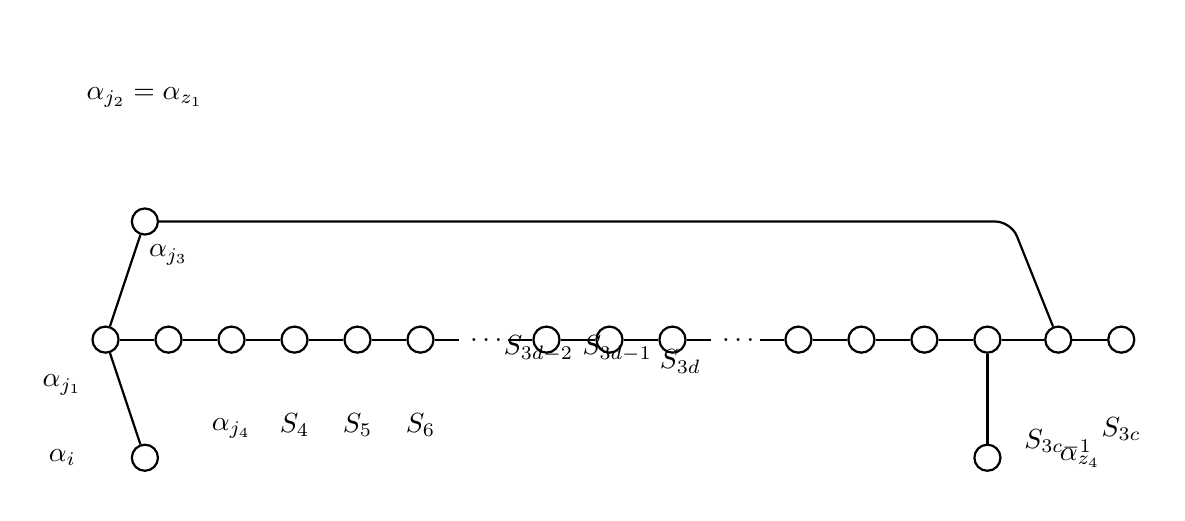
\begin{tikzpicture}
% \node[draw=none] (casenumber) at (-1.2, 3.0) {\emph{Case 3}};
\begin{scope}[every node/.style={circle,draw, minimum size=2.4mm}, xscale=1.0]
    \node[thick, circle, label={[label distance=0.5cm]180:$\alpha_{i}$}] (ai) at (1,0.5) {};
    \node[thick, circle, label={[label distance=0.5cm]90:$\alpha_{j_2}=\alpha_{z_1}$}] (aj2) at (1,3.5) {};
    \node[thick, circle, label={[shift={(-0.55, -1.2)}]:$\alpha_{j_1}$}] (aj1) at (0.5,2) {};
    \node[thick, circle, label={[label distance=0.45cm]90:$\alpha_{j_3}$}] (aj3) at (1.3,2) {};
    \node[thick, circle, label={[label distance=0.5cm]270:$\alpha_{j_4}$}] (aj4) at (2.1,2) {};
    
    \node[thick, circle, label={[label distance=0.5cm]270:$S_4$}] (s4) at (2.9,2) {};
    \node[thick, circle, label={[label distance=0.5cm]270:$S_5$}] (s5) at (3.7,2) {};
    \node[thick, circle, label={[label distance=0.5cm]270:$S_6$}] (s6) at (4.5,2) {};
    
    \node[rectangle, white, text=black, fill=white, minimum width=6mm, minimum height=12mm, inner sep=0.5mm] (dots1) at (5.3,2) {$\hspace{2pt}\dots$};
    
    \node[thick, circle, label={[shift={(-0.1, -0.925)}]:$S_{3d-2}$}] (s3d2) at (6.1,2) {};
    \node[thick, circle, label={[shift={(0.1, -0.925)}]:$S_{3d-1}$}] (s3d1) at (6.9,2) {};
    \node[thick, circle, label={[shift={(0.1, -0.925)}]:$S_{3d}$}] (s3d) at (7.7,2) {};
    
    \node[rectangle, white, text=black, fill=white, minimum width=6mm, minimum height=12mm, inner sep=0.5mm] (dots2) at (8.5,2) {$\hspace{2pt}\dots$};
    
    \node[thick, circle, label={[shift={(0.1, -1.5)}]}] (s3c5) at (9.3,2) {};
    \node[thick, circle, label={[shift={(0.3, -1.5)}]}] (s3c4) at (10.1,2) {};
    \node[thick, circle, label={[shift={(0.5, -1.5)}]}] (s3c3) at (10.9,2) {};
    
    \node[thick, circle, label={[label distance=0.55cm]0:$\alpha_{z_4}$}] (az4) at (11.7,0.5) {};
    
    \node[thick, circle, label={[shift={(0.5, -1.5)}]}] (s3c2) at (11.7,2) {};
    \node[thick, circle, label={[label distance=0.5cm]270:$S_{3c-1}$}] (s3c1) at (12.6,2) {};
    \node[thick, circle, label={[label distance=0.5cm]270:$S_{3c}$}] (s3c) at (13.4,2) {};
    
    \node[draw=none, inner sep=0, minimum size=0] (s3by) at (12.0, 3.5]) {};
    
    \draw [thick, rounded corners=2mm] (aj2.east)--(s3by.center)--(s3c1);
    
    \dashedcontainerthing{ai,aj1,aj3};
    \dashedcontainerthing{aj4,s4,s5};
    \dashedcontainerthing{aj4,s4,s5};
    \dashedcontainerthing{s6,s3d2,s3d1};
    \dashedcontainerthing{s3d,s3c5,s3c4};
    \dashedcontainerthing{s3c3,s3c2,az4,s3c2};
    \dashedcontainerthing{s3c,s3c1,s3by,aj2,s3by,s3c1};
\end{scope}
\begin{scope}
    \foreach \from/\to in {aj2/aj1, aj1/ai, aj1/aj3, aj3/aj4, aj4/s4, s4/s5, s5/s6, s6/dots1, dots1/s3d2, s3d2/s3d1, s3d1/s3d, s3d/dots2, dots2/s3c5, s3c5/s3c4, s3c4/s3c3, s3c3/s3c2, s3c2/s3c1, s3c1/s3c, az4/s3c2}
        \draw [thick] (\from) -- (\to);
\end{scope}
\end{tikzpicture}
    \caption{The structure of $M'$ in Construction~3} 
    \label{fig:threed_sr_as_symmetric_binary_repair_algorithm_7_cases_case_3}
\end{figure}
We first claim that $c > 1$. Suppose for a contradiction that $c = 1$. By the pseudocode, in Construction~3 it must be that $\alpha_{z_1} = \alpha_{j_2}$ and $v_{\alpha_{z_1}}(S_{3c-1})=1$. Since $c = 1$ it must be that $S_{3c-1}=\alpha_{j_3}$ so the triple $\{ \alpha_{j_1}, \alpha_{j_2}, \alpha_{j_3} \}$ forms a triangle in $(N, V)$, which contradicts the assumption that $(N, V)$ is triangle-free.

Since $c>1$ it follows that $c'=c-1$ is the value of $c$ in the second last iteration of the while loop. Consider the second-to-last iteration of the while loop. In this iteration, the subroutine identified some $\alpha_{w_1} = S_{3c-2}$ where $v_{S_{3c'}}(\alpha_{w_1})=1$, $\alpha_{w_1}\notin S$ and there existed some $\alpha_{z_3}\in N\setminus \{ \alpha_i \}$ where $v_{\alpha_{w_1}}(\alpha_{z_3})=1$ and $u_{\alpha_{z_3}}(M) = 0$. We shall identify the agent labelled $\alpha_{z_3}$ in this iteration as $\alpha_{z_4}$. It follows that $\alpha_{z_4} \neq \alpha_i$, $v_{S_{3c - 2}}(\alpha_{z_4}) = 1$, and $u_{\alpha_{z_4}}(M)=0$.

We claim that in $\alpha_{z_4} \neq \alpha_{j_2}$ since otherwise the triple $\{ \alpha_{z_4}, S_{3c-1}, S_{3c-2} \}$ forms a triangle in $(N, V)$, which contradicts the fact that $(N, V)$ is triangle-free. It follows that $\alpha_{z_4} \in N\setminus \{ \alpha_i, \alpha_{j_2} \}$, which completes the proof.
\end{proof}

Likewise in Construction~6, the subroutine identifies some agent $\alpha_{z_5}$ in $N\setminus \{ \alpha_i, \alpha_{j_2} \}$ exists where $v_{S_{3b+1}}(\alpha_{z_5})=1$ and $u_{\alpha_{z_5}}(M)=0$. Proposition~\ref{prop:threed_sr_as_symmetric_binary_az5exists} shows that such an agent must exist.

\begin{prop}
\label{prop:threed_sr_as_symmetric_binary_az5exists}
In Construction~6 of Subroutine~\algorithmfont{repair}, some agent $\alpha_{z_5}$ in $N\setminus \{ \alpha_i, \alpha_{j_2} \}$ exists where $v_{S_{3b+1}}(\alpha_{z_5})=1$ and $u_{\alpha_{z_5}}(M)=0$.
\end{prop}
\begin{proof}
Refer to Figure~\ref{fig:threed_sr_as_symmetric_binary_repair_algorithm_7_cases_case_6}. Consider the final value of $b$ in the subroutine. By the definition of $b$ and the pseudocode relating to Construction~6 it must be that $b < c$.

\begin{figure}
    \centering
    
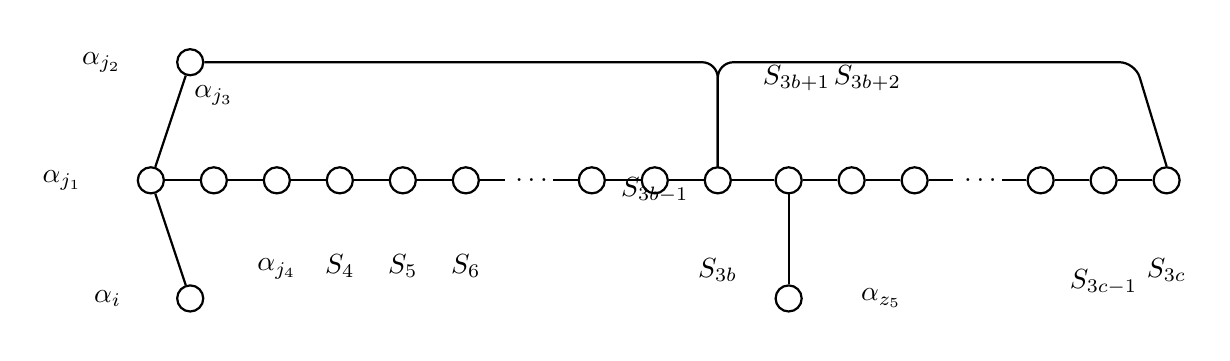
\begin{tikzpicture}
% \node[draw=none] (casenumber) at (-1.5, 3.0) {\emph{Case 6}};
\begin{scope}[every node/.style={circle,draw, minimum size=2.4mm}, xscale=1.0]
    \node[thick, circle, label={[label distance=0.5cm]180:$\alpha_{i}$}] (ai) at (1,0.5) {};
    \node[thick, circle, label={[label distance=0.5cm]180:$\alpha_{j_2}$}] (aj2) at (1,3.5) {};
    % \node[circle, densely dashed, minimum size=8mm] at (aj2) {};
    \node[thick, circle, label={[label distance=0.5cm]180:$\alpha_{j_1}$}] (aj1) at (0.5,2) {};
    \node[thick, circle, label={[label distance=0.45cm]90:$\alpha_{j_3}$}] (aj3) at (1.3,2) {};
    \node[thick, circle, label={[label distance=0.5cm]270:$\alpha_{j_4}$}] (aj4) at (2.1,2) {};
    
    \node[thick, circle, label={[label distance=0.5cm]270:$S_4$}] (s4) at (2.9,2) {};
    \node[thick, circle, label={[label distance=0.5cm]270:$S_5$}] (s5) at (3.7,2) {};
    \node[thick, circle, label={[label distance=0.5cm]270:$S_6$}] (s6) at (4.5,2) {};
    
    \node[rectangle, white, text=black, fill=white, minimum width=6mm, minimum height=12mm, inner sep=0.5mm] (dots1) at (5.3,2) {\hspace{2pt}$\dots$};
    
    \node[thick, circle, label={[shift={(0.1, -1.5)}]}] (s3b2) at (6.1,2) {};
    \node[thick, circle, label={[shift={(0.0, -0.925)}]:$S_{3b-1}$}] (s3b1) at (6.9,2) {};
    \node[draw=none] (s3b) at (7.7,2) {};
    
    \node[thick, circle, label={[shift={(0.1, 0.5)}]:$S_{3b+1}$}] (s3bp1) at (8.6,2) {};
    \node[thick, circle, label={[shift={(0.2, 0.5)}]:$S_{3b+2}$}] (s3bp2) at (9.4,2) {};
    \node[thick, circle, label={[shift={(0.5, -0.1)}]}] (s3bp3) at (10.2,2) {};
    
    \node[thick, circle, label={[label distance=0.55cm]0:$\alpha_{z_5}$}] (az5) at (8.6,0.5) {};
    
     \node[rectangle, white, text=black, fill=white, minimum width=6mm, minimum height=12mm, inner sep=0.5mm] (dots2) at (11.0,2) {\hspace{2pt}$\dots$};
    
    \node[thick, circle, label={[shift={(0.1, -1.5)}]}] (s3c2) at (11.8,2) {};
    \node[thick, circle, label={[label distance=0.5cm]270:$S_{3c-1}$}] (s3c1) at (12.6,2) {};
    \node[thick, circle, label={[label distance=0.5cm]270:$S_{3c}$}] (s3c) at (13.4,2) {};
    
    \node[draw=none, inner sep=0, minimum size=0] (s3bx) at (7.7, 3.5) {};
    \node[draw=none, inner sep=0, minimum size=0] (s3by) at (13.0, 3.5) {};
    
    \begin{scope}
    % \draw[thick, densely dashed] \convexpath{ai, aj1, aj3};
    
    \dashedcontainerthing{ai, aj1, aj3};
    \dashedcontainerthing{s3b,s3bx,s3by,s3c,s3by,s3bx,aj2,s3bx};
    \dashedcontainerthing{aj4,s4,s5};
    \dashedcontainerthing{az5,s3bp1,s3bp2,s3bp1};
    \dashedcontainerthing{s6,s3b2,s3b1};
    \dashedcontainerthing{s3c1,s3c2,s3bp3};
    \end{scope}
    
    \node[thick, circle,label={[label distance=0.5cm]270:$S_{3b}$}] (s3bextra) at (7.7,2) {};
    
    \draw [thick, rounded corners=2mm] (s3b)--(s3bx.center)--(s3by.center)--(s3c.north);
    \draw [thick, rounded corners=2mm] (s3b)--(s3bx.center)--(aj2);
    % \draw [thick, rounded corners=4mm] (s3b)--(s3bx)--(aj2);
\end{scope}
\begin{scope}
    \foreach \from/\to in {aj2/aj1, aj1/ai, aj1/aj3, aj3/aj4, aj4/s4, s4/s5, s5/s6, s6/dots1, dots1/s3b2, s3b2/s3b1, s3b1/s3b, s3b/s3bp1, s3bp1/s3bp2, s3bp2/s3bp3, s3bp3/dots2, dots2/s3c2, s3c2/s3c1, s3c1/s3c, s3bp1/az5}
        \draw [thick] (\from) -- (\to);
\end{scope}
\end{tikzpicture}
    \caption{The structure of $M'$ in Construction~6} 
    \label{fig:threed_sr_as_symmetric_binary_repair_algorithm_7_cases_case_6}
\end{figure}

Consider the $b\textsuperscript{th}$ iteration of the while loop. Since $b < c$, it must be that this iteration was not the final iteration. It follows that at the end of this iteration the subroutine identified some agent $\alpha_{w_1}=S_{3b+1}$ and then appended $\langle S_{3b+1}, S_{3b+2}, S_{3b+3} \rangle$ to the end of $S$. It also follows that, in this iteration, it also identified some agent $\alpha_{w_1}$ where there exists some $\alpha_{z_3} \in N \setminus \{ \alpha_i \}$ such that $v_{\alpha_{w_1}}(\alpha_{z_3})=1$ and $u_{\alpha_{z_3}}(M)=0$. We shall identify the agent labelled $\alpha_{z_3}$ in this iteration as $\alpha_{z_5}$. It follows that $\alpha_{z_5} \neq \alpha_i$, $v_{S_{3b + 1}}(\alpha_{z_5}) = 1$, and $u_{\alpha_{z_5}}(M)=0$.

We claim that in $\alpha_{z_5} \neq \alpha_{j_2}$. By the definition of $b$, it must be that $v_{S_{3b}}(\alpha_{j_2}) = 1$. Thus, if $\alpha_{z_5} = \alpha_{j_2}$ then the triple $\{ \alpha_{z_5}, S_{3b+1}, S_{3b} \}$ forms a triangle in $(N, V)$, which contradicts the fact that $(N, V)$ is triangle-free. It follows that $\alpha_{z_5} \in N\setminus \{ \alpha_i, \alpha_{j_2} \}$, which completes the proof.
\end{proof}

\begin{lem}
\label{lem:threed_sr_as_symmetric_binary_algreturnspmatching}
Subroutine~\algorithmfont{repair} returns a $P$\nobreakdash-matching.
\end{lem}
\begin{proof}
By the construction of $M'$ in Constructions 1--7 of $M'$, shown in Figures~\ref{fig:threed_sr_as_symmetric_binary_repair_algorithm_7_cases_case_1}\nobreakdash--\ref{fig:threed_sr_as_symmetric_binary_repair_algorithm_7_cases_case_7}.
\end{proof}

In Lemmas~\ref{lem:threed_sr_as_symmetric_binary_algocases1and3noalphapexists}, \ref{lem:threed_sr_as_symmetric_binary_algocases245and6noalphapexists} and~\ref{lem:threed_sr_as_symmetric_binary_algocase7noalphapexists} we show that in no construction of $M'$ does there exist any agent $\alpha_g$ where where $u_{\alpha_{g}}(M') < u_{\alpha_{g}}(M)$ and $\alpha_g$ belongs to a triple that blocks $M'$. This fact will help us show that $M'$ must be stable.

\begin{lem}
\label{lem:threed_sr_as_symmetric_binary_algocases1and3noalphapexists}
In Constructions 1 and 3 of Subroutine~\algorithmfont{repair}, there exists no agent $\alpha_{g}$ where $u_{\alpha_{g}}(M') < u_{\alpha_{g}}(M)$ and $\alpha_g$ belongs to a triple that blocks $M'$.
\end{lem}
\begin{proof}
Refer to Figures~\ref{fig:threed_sr_as_symmetric_binary_repair_algorithm_7_cases_case_3} and~\ref{fig:threed_sr_as_symmetric_binary_repair_algorithm_7_cases_case_1}. Suppose for a contradiction that there exists some such $\alpha_g\in N$. By the construction of $M'$ in Constructions 1 and 3, $u_{\alpha_p}(M')\geq u_{\alpha_p}(M)$ for any $\alpha_p\in N \setminus S$. It follows that $\alpha_g\in S$ and thus by the construction of $M'$ in Constructions 1 and 3 that $u_{\alpha_g}(M')\geq 1$. Since $u_{\alpha_{g}}(M') < u_{\alpha_{g}}(M)$ by assumption it must be that $u_{\alpha_g}(M) = 2$. The only such agents in $S$ are labelled $S_{3d-1}$ for some $d$ where $1 \leq d \leq c$, so it must be that $\alpha_g = S_{3d-1}$ for some such $d$. 

\begin{figure}
    \centering
    
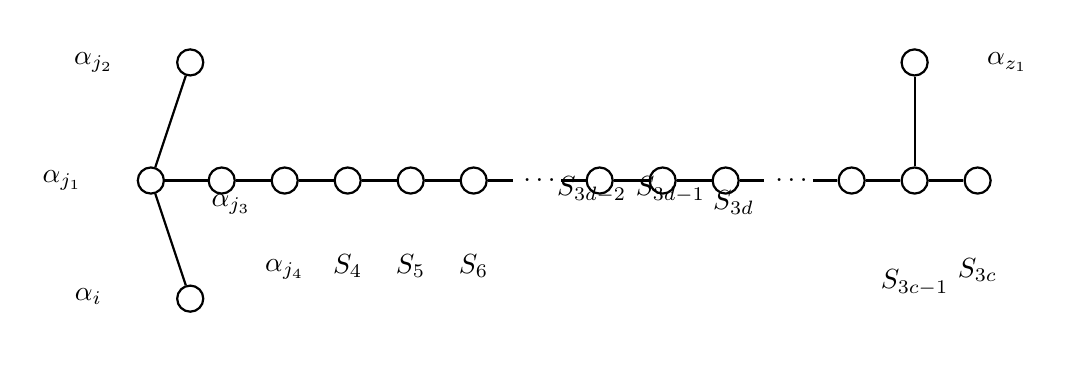
\begin{tikzpicture}
% \draw[help lines,step=1] (0,0) grid (10,4);
% \node[draw=none] (casenumber) at (-1.5, 3.0) {\emph{Case 1}};
\begin{scope}[every node/.style={circle,draw, minimum size=2.4mm}, xscale=1.0]
    \node[thick, circle, label={[label distance=0.5cm]180:$\alpha_{i\phantom{j_2}}$}] (ai) at (1,0.5) {};
    \node[thick, circle, label={[label distance=0.6cm]180:$\alpha_{j_2}$}] (aj2) at (1,3.5) {};
    \node[thick, circle, label={[label distance=0.5cm]180:$\alpha_{j_1}$}] (aj1) at (0.5,2) {};
    \node[thick, circle, label={[shift={(0.12, -0.925)}]:$\alpha_{j_3}$}] (aj3) at (1.4,2) {};
    \node[thick, circle, label={[label distance=0.5cm]270:$\alpha_{j_4}$}] (aj4) at (2.2,2) {};
    \node[thick, circle, label={[label distance=0.5cm]270:$S_{4}$}] (s4) at (3.0,2) {};
    \node[thick, circle, label={[label distance=0.5cm]270:$S_{5}$}] (s5) at (3.8,2) {};
    \node[thick, circle, label={[label distance=0.5cm]270:$S_{6}$}] (s6) at (4.6,2) {};
    \node[rectangle, white, text=black, fill=white, minimum width=6mm, minimum height=12mm, inner sep=0.5mm] (dots1) at (5.4,2) {\hspace{2pt}$\dots$};
    \node[thick, circle, label={[shift={(-0.1, -0.925)}]:$S_{3d-2}$}] (s3d2) at (6.2,2) {};
    \node[thick, circle, label={[shift={(0.1, -0.925)}]:$S_{3d-1}$}] (s3d1) at (7.0,2) {};
    \node[thick, circle, label={[shift={(0.1, -0.925)}]:$S_{3d}$}] (s3d) at (7.8,2) {};
    \node[rectangle, white, text=black, fill=white, minimum width=6mm, minimum height=12mm, inner sep=0.5mm] (dots2) at (8.6,2) {\hspace{2pt}$\dots$};
    \node[thick, circle] (s3c2) at (9.4,2) {};
    \node[thick, circle, label={[label distance=0.5cm]270:$S_{3c-1}$}] (s3c1) at (10.2,2) {};
    \node[thick, circle, label={[label distance=0.5cm]270:$S_{3c}$}] (s3c) at (11.0,2) {};
    \node[thick, circle, label={[label distance=0.55cm]0:$\alpha_{z_1}$}] (az1) at (10.2,3.5) {};
    
    \dashedcontainerthing{ai,aj1,aj2,aj1};
    \dashedcontainerthing{aj3,aj4,s4};
    \dashedcontainerthing{s5,s6,s3d2};
    \dashedcontainerthing{s3d1,s3d,s3c2};
    \dashedcontainerthing{az1,s3c1,s3c,s3c1};
\end{scope}
\begin{scope}
    \foreach \from/\to in {aj2/aj1, aj1/ai, aj1/aj3, aj3/aj4, aj4/s4, s4/s5, s5/s6, s6/dots1, dots1/s3d2, s3d2/s3d1, s3d1/s3d, s3d/dots2, dots2/s3c2, s3c2/s3c1, s3c1/s3c, s3c1/az1}
        \draw [thick] (\from) -- (\to);
\end{scope}
\end{tikzpicture}
    \caption{The structure of $M'$ in Construction~1} 
    \label{fig:threed_sr_as_symmetric_binary_repair_algorithm_7_cases_case_1}
\end{figure}

First consider $S_{3c-1}$. Since $u_{S_{3c-1}}(M')=2$ it follows that $S_{3c-1}$ does not belong to a triple that blocks $M'$ and hence $\alpha_g\neq S_{3c-1}$. It remains that $\alpha_g = S_{3d-1}$ where $1\leq d < c$. By assumption, it must be that some triple $\{ S_{3d-1}, \alpha_{k_1}, \alpha_{k_2} \}$ blocks $M'$, where $\alpha_{k_1}, \alpha_{k_2} \in N$. Since $u_{S_{3d-1}}(M')=1$ it follows that $u_{S_{3d-1}}(\{ \alpha_{k_1}, \alpha_{k_2} \})=2$ and thus that $v_{S_{3d-1}}(\alpha_{k_1})=v_{S_{3d-1}}(\alpha_{k_2})=1$. Consider $\alpha_{k_1}$ and $\alpha_{k_2}$. Since $(N, V)$ is triangle-free, it must be that $v_{\alpha_{k_1}}(\alpha_{k_2}) = 0$ and thus that $u_{\alpha_{k_1}}(\{ S_{3d-1}, \alpha_{k_2} \})=u_{\alpha_{k_2}}(\{ S_{3d-1}, \alpha_{k_1} \})=1$. Since the triple $\{ S_{3d-1}, \alpha_{k_1}, \alpha_{k_2} \}$ blocks $M'$ it follows that $u_{\alpha_{k_1}}(M')=u_{\alpha_{k_2}}(M')=0$. By the construction of $M'$, there exists no $\alpha_p \in N$ where $u_{\alpha_p}(M') = 0$ and $u_{\alpha_p}(M') < u_{\alpha_p}(M)$. It follows that $u_{\alpha_{k_1}}(M)=u_{\alpha_{k_2}}(M)=0$. Recall the $d\textsuperscript{th}$ iteration of the while loop. We have shown that two agents $\alpha_{k_1}, \alpha_{k_2}$ exist in that iteration such that $v_{S_{3d-1}}(\alpha_{k_1})=v_{S_{3d-1}}(\alpha_{k_2})=1$ and $u_{\alpha_{k_1}}(M)=u_{\alpha_{k_2}}(M)=0$. It follows that, in that iteration, there existed some $\alpha_{z_1} \in N\setminus \{\alpha_i\}$ where $v_{\alpha_{z_1}}(S_{3d-1})=1$ and $u_{\alpha_{z_1}}(M)=0$, since either $\alpha_{z_1}=\alpha_{k_1}$ or $\alpha_{i}=\alpha_{k_1}$ and $\alpha_{z_1}=\alpha_{k_2}$. In that iteration, since $\alpha_{z_1}\neq \bot$ the break condition held and the while loop terminated. This is a contradiction since $d < c$.
\end{proof}

\begin{lem}
\label{lem:threed_sr_as_symmetric_binary_algocases245and6noalphapexists}
In Constructions 2, 4, 5, and 6 of Subroutine~\algorithmfont{repair}, there exists no agent $\alpha_{g}$ where $u_{\alpha_{g}}(M') < u_{\alpha_{g}}(M)$ and $\alpha_g$ belongs to a triple that blocks $M'$.
\end{lem}
\begin{proof}
Refer to Figures~\ref{fig:threed_sr_as_symmetric_binary_repair_algorithm_7_cases_case_6}, \ref{fig:threed_sr_as_symmetric_binary_repair_algorithm_7_cases_case_2}, \ref{fig:threed_sr_as_symmetric_binary_repair_algorithm_7_cases_case_4}, and~\ref{fig:threed_sr_as_symmetric_binary_repair_algorithm_7_cases_case_5}. Suppose for a contradiction that there exists some such $\alpha_g\in N$. By the construction of $M'$ in Constructions 2, 4, 5, and 6, $u_{\alpha_p}(M')\geq u_{\alpha_p}(M)$ for any $\alpha_p\in N \setminus S$. It follows that $\alpha_g \in S$ and hence $u_{\alpha_g}(M')\geq 1$. Since $u_{\alpha_{g}}(M') < u_{\alpha_{g}}(M)$ it must be that $u_{\alpha_g}(M) = 2$. The only such agents in $S$ are labelled $S_{3d-1}$ for some $d$ where $1 \leq d \leq c$, so it must be that $\alpha_g = S_{3d-1}$ for some such $d$. 

\begin{figure}
    \centering
    


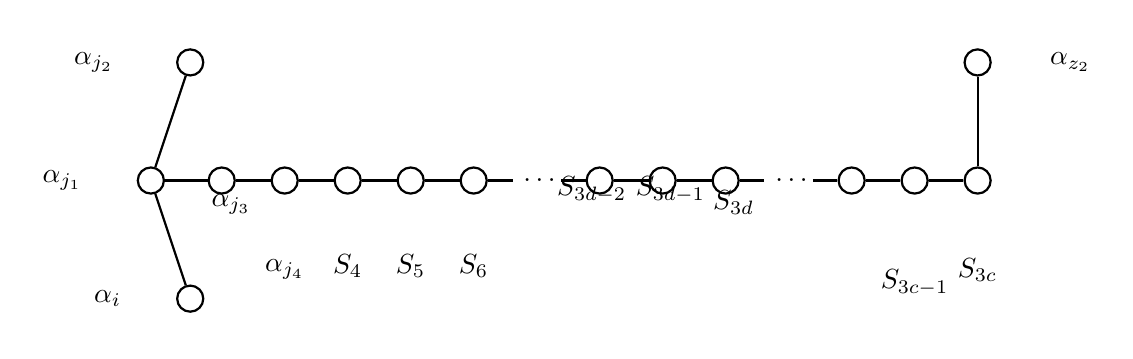
\begin{tikzpicture}
% \node[draw=none] (casenumber) at (-1.5, 3.0) {\emph{Case 2}};
\begin{scope}[every node/.style={circle,draw, minimum size=2.4mm}, xscale=1.0]
    \node[thick, circle, label={[label distance=0.5cm]180:$\alpha_{i}$}] (ai) at (1,0.5) {};
    \node[thick, circle, label={[label distance=0.6cm]180:$\alpha_{j_2}$}] (aj2) at (1,3.5) {};
    \node[thick, circle, label={[label distance=0.5cm]180:$\alpha_{j_1}$}] (aj1) at (0.5,2) {};
    \node[thick, circle, label={[shift={(0.12, -0.925)}]:$\alpha_{j_3}$}] (aj3) at (1.4,2) {};
    \node[thick, circle, label={[label distance=0.5cm]270:$\alpha_{j_4}$}] (aj4) at (2.2,2) {};
    \node[thick, circle, label={[label distance=0.5cm]270:$S_{4}$}] (s4) at (3.0,2) {};
    \node[thick, circle, label={[label distance=0.5cm]270:$S_{5}$}] (s5) at (3.8,2) {};
    \node[thick, circle, label={[label distance=0.5cm]270:$S_{6}$}] (s6) at (4.6,2) {};
    \node[rectangle, white, text=black, fill=white, minimum width=6mm, minimum height=12mm, inner sep=0.5mm] (dots1) at (5.4,2) {\hspace{2pt}$\dots$};
    \node[thick, circle, label={[shift={(-0.1, -0.925)}]:$S_{3d-2}$}] (s3d2) at (6.2,2) {};
    \node[thick, circle, label={[shift={(0.1, -0.925)}]:$S_{3d-1}$}] (s3d1) at (7.0,2) {};
    \node[thick, circle, label={[shift={(0.1, -0.925)}]:$S_{3d}$}] (s3d) at (7.8,2) {};
    \node[rectangle, white, text=black, fill=white, minimum width=6mm, minimum height=12mm, inner sep=0.5mm] (dots2) at (8.6,2) {\hspace{2pt}$\dots$};
    \node[thick, circle] (s3c2) at (9.4,2) {};
    \node[thick, circle, label={[label distance=0.5cm]270:$S_{3c-1}$}] (s3c1) at (10.2,2) {};
    \node[thick, circle, label={[label distance=0.5cm]270:$S_{3c}$}] (s3c) at (11.0,2) {};
    
    \node[thick, circle, label={[label distance=0.55cm]0:$\alpha_{z_2}$}] (az2) at (11.0,3.5) {};
    
    \dashedcontainerthing{ai,aj1,aj2,aj1};
    \dashedcontainerthing{aj3,aj4,s4};
    \dashedcontainerthing{s5,s6,s3d2};
    \dashedcontainerthing{s3d1,s3d,s3c2};
    \dashedcontainerthing{s3c1,s3c,az2,s3c};
\end{scope}
\begin{scope}
    \foreach \from/\to in {aj2/aj1, aj1/ai, aj1/aj3, aj3/aj4, aj4/s4, s4/s5, s5/s6, s6/dots1, dots1/s3d2, s3d2/s3d1, s3d1/s3d, s3d/dots2, dots2/s3c2, s3c2/s3c1, s3c1/s3c, s3c/az2}
        \draw [thick] (\from) -- (\to);
\end{scope}
\end{tikzpicture}
    \caption{The structure of $M'$ in Construction~2} 
    \label{fig:threed_sr_as_symmetric_binary_repair_algorithm_7_cases_case_2}
\end{figure}

\begin{figure}
    \centering
    

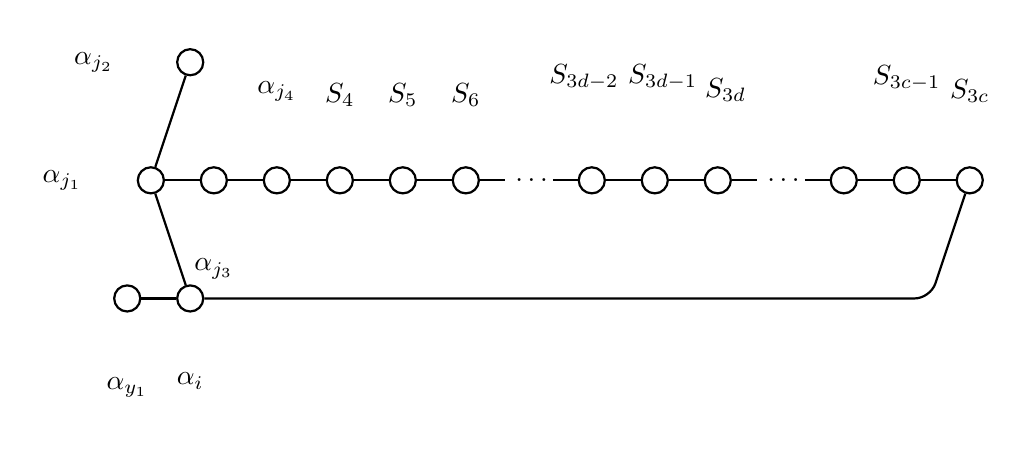
\begin{tikzpicture}
% \node[draw=none] (casenumber) at (-1.5, 3.0) {\emph{Case 4}};
\begin{scope}[every node/.style={circle,draw, minimum size=2.4mm}, xscale=1.0]
    \node[thick, circle, label={[label distance=0.5cm]270:$\alpha_{i}$}] (ai) at (1,0.5) {};
    \node[thick, circle, label={[label distance=0.6cm]180:$\alpha_{j_2}$}] (aj2) at (1,3.5) {};
    \node[thick, circle, label={[label distance=0.5cm]180:$\alpha_{j_1}$}] (aj1) at (0.5,2) {};
    \node[thick, circle, label={[label distance=0.5cm]270:$\alpha_{j_3}$}] (aj3) at (1.3,2) {};
    \node[thick, circle, label={[label distance=0.5cm]90:$\alpha_{j_4}$}] (aj4) at (2.1,2) {};
    
    \node[thick, circle, label={[label distance=0.5cm]270:$\alpha_{y_1}$}] (ay1) at (0.2,0.5) {};
    
    \node[thick, circle, label={[label distance=0.5cm]90:$S_4$}] (s4) at (2.9,2) {};
    \node[thick, circle, label={[label distance=0.5cm]90:$S_5$}] (s5) at (3.7,2) {};
    \node[thick, circle, label={[label distance=0.5cm]90:$S_6$}] (s6) at (4.5,2) {};
    
    \node[rectangle, white, text=black, fill=white, minimum width=6mm, minimum height=12mm, inner sep=0.5mm] (dots1) at (5.3,2) {\hspace{2pt}$\dots$};
    
    \node[thick, circle, label={[shift={(-0.1, 0.5)}]:$S_{3d-2}$}] (s3d2) at (6.1,2) {};
    \node[thick, circle, label={[shift={(0.1, 0.5)}]:$S_{3d-1}$}] (s3d1) at (6.9,2) {};
    \node[thick, circle, label={[shift={(0.1, 0.5)}]:$S_{3d}$}] (s3d) at (7.7,2) {};
    
    \node[rectangle, white, text=black, fill=white, minimum width=6mm, minimum height=10mm, inner sep=0.5mm] (dots2) at (8.5,2) {\hspace{2pt}$\dots$};
    
    \node[thick, circle, label={[shift={(0.1, -1.5)}]}] (s3c2) at (9.3,2) {};
    \node[thick, circle, label={[label distance=0.5cm]90:$S_{3c-1}$}] (s3c1) at (10.1,2) {};
    \node[thick, circle, label={[label distance=0.5cm]90:$S_{3c}$}] (s3c) at (10.9,2) {};
    
    \node[draw=none, inner sep=0, minimum size=0] (s3by) at (10.4, 0.5]) {};
    
    \draw [thick, rounded corners=2mm] (ai.east)--(s3by.center)--(s3c);
    
    \dashedcontainerthing{aj1,aj2,aj3};
    \dashedcontainerthing{aj4,s4,s5};
    \dashedcontainerthing{s6,s3d2,s3d1};
    \dashedcontainerthing{s3d,s3c2,s3c1};
    \dashedcontainerthing{s3c,s3by,ai,ay1,ai,s3by,s3c};
\end{scope}
\begin{scope}
    \foreach \from/\to in {aj2/aj1, aj1/ai, aj1/aj3, aj3/aj4, aj4/s4, s4/s5, s5/s6, s6/dots1, dots1/s3d2, s3d2/s3d1, s3d1/s3d, s3d/dots2, dots2/s3c2, s3c2/s3c1, s3c1/s3c, ay1/ai}
        \draw [thick] (\from) -- (\to);
\end{scope}
\end{tikzpicture}
    \caption{The structure of $M'$ in Construction~4} 
    \label{fig:threed_sr_as_symmetric_binary_repair_algorithm_7_cases_case_4}
\end{figure}

\begin{figure}
    \centering
    

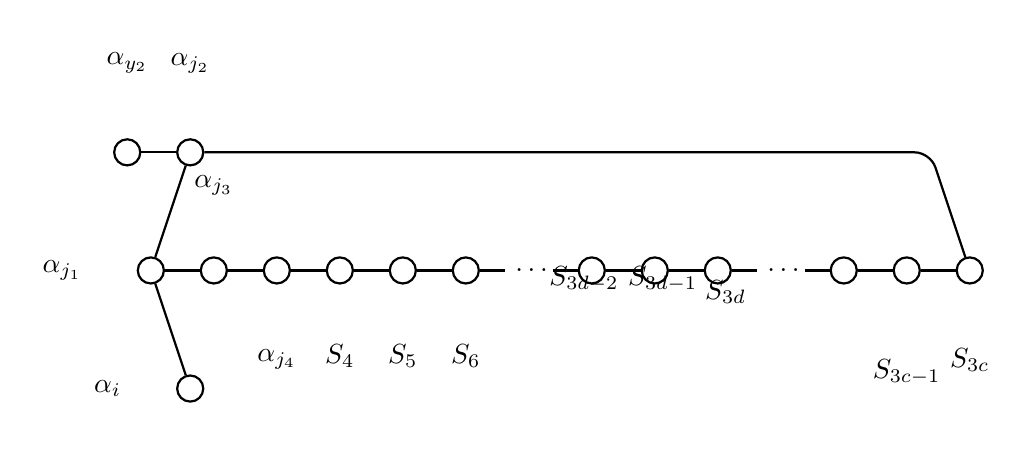
\begin{tikzpicture}
% \node[draw=none] (casenumber) at (-1.5, 3.0) {\emph{Case 5}};
\begin{scope}[every node/.style={circle,draw, minimum size=2.4mm}, xscale=1.0]
    \node[thick, circle, label={[label distance=0.5cm]180:$\alpha_{i}$}] (ai) at (1,0.5) {};
    \node[thick, circle, label={[label distance=0.5cm]90:$\alpha_{j_2}$}] (aj2) at (1,3.5) {};
    \node[thick, circle, label={[label distance=0.5cm]180:$\alpha_{j_1}$}] (aj1) at (0.5,2) {};
    \node[thick, circle, label={[label distance=0.45cm]90:$\alpha_{j_3}$}] (aj3) at (1.3,2) {};
    \node[thick, circle, label={[label distance=0.5cm]270:$\alpha_{j_4}$}] (aj4) at (2.1,2) {};
    
    \node[thick, circle, label={[label distance=0.5cm]90:$\alpha_{y_2}$}] (ay2) at (0.2,3.5) {};
    
    \node[thick, circle, label={[label distance=0.5cm]270:$S_4$}] (s4) at (2.9,2) {};
    \node[thick, circle, label={[label distance=0.5cm]270:$S_5$}] (s5) at (3.7,2) {};
    \node[thick, circle, label={[label distance=0.5cm]270:$S_6$}] (s6) at (4.5,2) {};
    
    \node[rectangle, white, text=black, fill=white, minimum width=6mm, minimum height=12mm, inner sep=0.5mm] (dots1) at (5.3,2) {\hspace{2pt}$\dots$};
    
    \node[thick, circle, label={[shift={(-0.1, -0.925)}]:$S_{3d-2}$}] (s3d2) at (6.1,2) {};
    \node[thick, circle, label={[shift={(0.1, -0.925)}]:$S_{3d-1}$}] (s3d1) at (6.9,2) {};
    \node[thick, circle, label={[shift={(0.1, -0.925)}]:$S_{3d}$}] (s3d) at (7.7,2) {};
    
    \node[rectangle, white, text=black, fill=white, minimum width=6mm, minimum height=12mm, inner sep=0.5mm] (dots2) at (8.5,2) {\hspace{2pt}$\dots$};
    
    \node[thick, circle, label={[shift={(0.1, -1.5)}]}] (s3c2) at (9.3,2) {};
    \node[thick, circle, label={[label distance=0.5cm]270:$S_{3c-1}$}] (s3c1) at (10.1,2) {};
    \node[thick, circle, label={[label distance=0.5cm]270:$S_{3c}$}] (s3c) at (10.9,2) {};
    
    \node[draw=none, inner sep=0, minimum size=0] (s3by) at (10.4, 3.5]) {};
    
    \draw [thick, rounded corners=2mm] (aj2.east)--(s3by.center)--(s3c);
    
    \dashedcontainerthing{ai,aj1,aj3};
    \dashedcontainerthing{aj4,s4,s5};
    \dashedcontainerthing{s6,s3d2,s3d1};
    \dashedcontainerthing{s3d,s3c2,s3c1};
    \dashedcontainerthing{s3c,s3by,aj2,ay2,aj2,s3by,s3c};
\end{scope}
\begin{scope}
    \foreach \from/\to in {aj2/aj1, aj1/ai, aj1/aj3, aj3/aj4, aj4/s4, s4/s5, s5/s6, s6/dots1, dots1/s3d2, s3d2/s3d1, s3d1/s3d, s3d/dots2, dots2/s3c2, s3c2/s3c1, s3c1/s3c, ay2/aj2}
        \draw [thick] (\from) -- (\to);
\end{scope}
\end{tikzpicture}
    \caption{The structure of $M'$ in Construction~5} 
    \label{fig:threed_sr_as_symmetric_binary_repair_algorithm_7_cases_case_5}
\end{figure}

Consider $S_{3d-1}$ for $1\leq d \leq c$. Note that in Constructions 2, 4, 5, and 6 it must be that $u_{S_{3d-1}}(M)=2$ and $u_{S_{3d-1}}(M')=1$. By assumption, it must be that some triple $\{ S_{3d-1}, \alpha_{k_1}, \alpha_{k_2} \}$ blocks $M'$, where $\alpha_{k_1}, \alpha_{k_2} \in N$. Since $u_{S_{3d-1}}(M')=1$ it follows that $u_{S_{3d-1}}(\{ \alpha_{k_1}, \alpha_{k_2} \})=2$. Consider $\alpha_{k_1}$ and $\alpha_{k_2}$. Since $(N, V)$ is triangle-free, it must be that $v_{\alpha_{k_1}}(\alpha_{k_2})=0$ and thus that $u_{\alpha_{k_1}}(\{ S_{3d-1}, \alpha_{k_2} \}) = u_{\alpha_{k_2}}(\{ S_{3d-1}, \alpha_{k_1} \}) = 1$. It follows that $u_{\alpha_{k_1}}(M') = u_{\alpha_{k_2}}(M') = 0$. By the construction of $M'$, there exists no $\alpha_p \in N$ where $u_{\alpha_p}(M') = 0$ and $u_{\alpha_p}(M') < u_{\alpha_p}(M)$. It follows that $u_{\alpha_{k_1}}(M)=u_{\alpha_{k_2}}(M)=0$. Recall the $d\textsuperscript{th}$ iteration of the while loop. We have shown that two agents $\alpha_{k_1}, \alpha_{k_2}$ exist where $v_{S_{3d-1}}(\alpha_{k_1})=v_{S_{3d-1}}(\alpha_{k_2})=1$ and $u_{\alpha_{k_1}}(M)=u_{\alpha_{k_2}}(M)=0$. It follows that, in that iteration, there existed some $\alpha_{z_1} \in N\setminus \{\alpha_i\}$ where $v_{\alpha_{z_1}}(S_{3d-1})=1$ and $u_{\alpha_{z_1}}(M)=0$, since either $\alpha_{z_1}=\alpha_{k_1}$ or $\alpha_{i}=\alpha_{k_1}$ and $\alpha_{z_1}=\alpha_{k_2}$. In that iteration, since $\alpha_{z_1}\neq \bot$ the break condition must have held, the while loop terminated, and the condition for either Construction~1 or Construction~3 was true. This is a contradiction since by assumption the subroutine constructed $M'$ according to one of Constructions 2, 4, 5, or 6.
\end{proof}

\begin{lem}
\label{lem:threed_sr_as_symmetric_binary_algocase7noalphapexists}
In Construction~7 of Subroutine~\algorithmfont{repair}, there exists no agent $\alpha_{g}$ where $u_{\alpha_{g}}(M') < u_{\alpha_{g}}(M)$ and $\alpha_g$ belongs to a triple that blocks $M'$.
\end{lem}
\begin{proof}

Refer to Figure~\ref{fig:threed_sr_as_symmetric_binary_repair_algorithm_7_cases_case_7}. Suppose for a contradiction that there exists some such $\alpha_g$.

\begin{figure}
    \centering
    


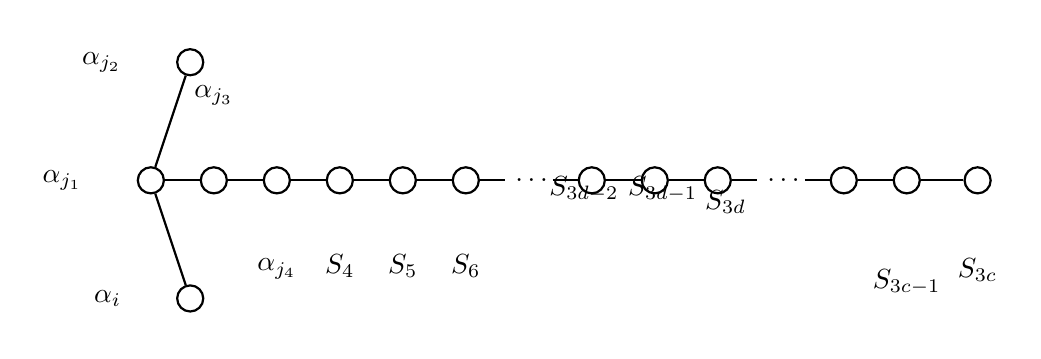
\begin{tikzpicture}
% \node[draw=none] (casenumber) at (-1.5, 3.0) {\emph{Case 7}};
\begin{scope}[every node/.style={circle,draw, minimum size=2.4mm}, xscale=1.0]
    \node[thick, circle, label={[label distance=0.5cm]180:$\alpha_{i}$}] (ai) at (1,0.5) {};
    \node[thick, circle, label={[label distance=0.5cm]180:$\alpha_{j_2}$}] (aj2) at (1,3.5) {};
    
    \node[thick, circle, label={[label distance=0.5cm]180:$\alpha_{j_1}$}] (aj1) at (0.5,2) {};
    \node[thick, circle, label={[label distance=0.45cm]90:$\alpha_{j_3}$}] (aj3) at (1.3,2) {};
    \node[thick, circle, label={[label distance=0.5cm]270:$\alpha_{j_4}$}] (aj4) at (2.1,2) {};
    
    \node[thick, circle, label={[label distance=0.5cm]270:$S_4$}] (s4) at (2.9,2) {};
    \node[thick, circle, label={[label distance=0.5cm]270:$S_5$}] (s5) at (3.7,2) {};
    \node[thick, circle, label={[label distance=0.5cm]270:$S_6$}] (s6) at (4.5,2) {};
    
    \node[rectangle, white, text=black, fill=white, minimum width=6mm, minimum height=12mm, inner sep=0.5mm] (dots1) at (5.3,2) {\hspace{2pt}$\dots$};
    
    \node[thick, circle, label={[shift={(-0.1, -0.925)}]:$S_{3d-2}$}] (s3d2) at (6.1,2) {};
    \node[thick, circle, label={[shift={(0.1, -0.925)}]:$S_{3d-1}$}] (s3d1) at (6.9,2) {};
    \node[thick, circle, label={[shift={(0.1, -0.925)}]:$S_{3d}$}] (s3d) at (7.7,2) {};
    
    \node[rectangle, white, text=black, fill=white, minimum width=6mm, minimum height=12mm, inner sep=0.5mm] (dots2) at (8.5,2) {\hspace{2pt}$\dots$};
    
    \node[thick, circle, label={[shift={(0.1, -1.5)}]}] (s3c2) at (9.3,2) {};
    \node[thick, circle, label={[label distance=0.5cm]270:$S_{3c-1}$}] (s3c1) at (10.1,2) {};
    \node[thick, circle, label={[label distance=0.5cm]270:$S_{3c}$}] (s3c) at (11.0,2) {};
    
    \dashedcontainerthing{aj2};
    \dashedcontainerthing{ai,aj1,aj3};
    \dashedcontainerthing{aj4,s4,s5};
    \dashedcontainerthing{s6,s3d2,s3d1};
    \dashedcontainerthing{s3d,s3c2,s3c1};
    \dashedcontainerthing{s3c};
\end{scope}
\begin{scope}
    \foreach \from/\to in {aj2/aj1, aj1/ai, aj1/aj3, aj3/aj4, aj4/s4, s4/s5, s5/s6, s6/dots1, dots1/s3d2, s3d2/s3d1, s3d1/s3d, s3d/dots2, dots2/s3c2, s3c2/s3c1, s3c1/s3c}
        \draw [thick] (\from) -- (\to);
\end{scope}
\end{tikzpicture}

    \caption{The structure of $M'$ in Construction~7} 
    \label{fig:threed_sr_as_symmetric_binary_repair_algorithm_7_cases_case_7}
\end{figure}

First, consider any $\alpha_p \in N$ where $\alpha_p \notin S \cup \{ \alpha_{j_2}, \alpha_{i} \}$. By the construction of $M'$, it can be seen that $M(\alpha_p)=M'(\alpha_p)$ so $u_{\alpha_p}(M)=u_{\alpha_p}(M')$ and thus $\alpha_g \notin S \cup \{ \alpha_{j_2}, \alpha_{i} \}$.

Next, consider $\alpha_i$ and $\alpha_{j_2}$. Since $u_{\alpha_i}(M) = 0 < 1 = u_{\alpha_i}(M')$ it follows that $\alpha_g \neq \alpha_i$.  Similarly, since $u_{\alpha_{j_2}}(M) = u_{\alpha_{j_2}}(M') = 0$ it follows that $\alpha_g \neq \alpha_{j_2}$.

It remains that $\alpha_g \in S$.

Consider any $S_{3d-2}$ where $1\leq d\leq c$. By construction of $M'$ it follows that $u_{S_{3d-2}}(M')=2$ so $\alpha_{p} \neq S_{3d-2}$ for any $d$ where $1\leq d\leq c$.

Next, consider any $S_{3d-1}$ where $1\leq d \leq c$. Suppose for a contradiction that $\alpha_g = S_{3d-1}$ where $1\leq d \leq c$ and thus that some triple $\{ S_{3d-1}, \alpha_{k_1}, \alpha_{k_2} \}$ blocks $M'$ where $\alpha_{k_1}, \alpha_{k_2} \in N$. Since $u_{S_{3d-1}}(M')=1$ it follows that $u_{S_{3d-1}}(\{ \alpha_{k_1}, \alpha_{k_2} \})=2$. Consider $\alpha_{k_1}$ and $\alpha_{k_2}$. Since $(N, V)$ is triangle-free, it must be that $v_{\alpha_{k_1}}(\alpha_{k_2}) = 0$ and thus that $u_{\alpha_{k_1}}(\{ S_{3d-1}, \alpha_{k_2} \})=u_{\alpha_{k_2}}(\{ S_{3d-1}, \alpha_{k_1} \})=1$. It follows that $u_{\alpha_{k_1}}(M')=u_{\alpha_{k_2}}(M')=0$. By construction of $M'$ it can be seen that $S_{3c}$ is the only agent $\alpha_p$ in $N$ where $u_{\alpha_p}(M')=0$ and $u_{\alpha_p}(M') < u_{\alpha_p}(M)$. Since the triple $\{ S_{3d-1}, \alpha_{k_1}, \alpha_{k_2} \}$ blocks $M'$ and $u_{\alpha_{k_1}}(\{ S_{3d-1}, \alpha_{k_2} \})=u_{\alpha_{k_2}}(\{ S_{3d-1}, \alpha_{k_1} \})=1$ it follows that either $u_{\alpha_{k_1}}(M)=0$, $u_{\alpha_{k_2}}(M)=0$, or both. Assume without loss of generality that $u_{\alpha_{k_1}}(M)=0$. Since $u_{\alpha_{k_1}}(M')=0$ it follows that $\alpha_{k_1}\neq \alpha_i$. Recall the $d\textsuperscript{th}$ iteration of the while loop. Since $v_{S_{3d-1}}(\alpha_{k_1})=1$, $u_{\alpha_{k_1}}(M)=0$, and $\alpha_{k_1}\neq \alpha_i$, it follows that, in that iteration, there existed some $\alpha_{z_1} \in N\setminus \{\alpha_i\}$, namely $\alpha_{k_1}$, where $v_{\alpha_{z_1}}(S_{3d-1})=1$ and $u_{\alpha_{z_1}}(M)=0$. In that iteration, since $\alpha_{z_1} \neq \bot$ the break condition must have held, the while loop terminated, and either the condition for Construction~1 was true or the condition for Construction~3 was true. This is a contradiction since by assumption the subroutine constructed $M'$ according to Construction~7. It follows that $\alpha_g \neq S_{3d-1}$ for any $d$ where $1\leq d \leq c$. 

Next, consider any $S_{3d}$ where $1\leq d < c$. By construction of $M'$ it follows that $u_{S_{3d}}(M')=u_{S_{3d}}(M)=1$ so $\alpha_{g} \neq S_{3d}$ for any such $d$.

The only possibility is thus that $\alpha_g = S_{3c}$. By the definition of $\alpha_g$, there exists some triple $\{ S_{3c}, \alpha_{k_1}, \alpha_{k_2} \}$ that blocks $M'$, where $\alpha_{k_1}, \alpha_{k_2} \in N$. Since $u_{S_{3c}}(M')=0$ it must be that either $v_{S_{3c}}(\alpha_{k_1})=1$, $v_{S_{3c}}(\alpha_{k_2})=1$, or both.

Firstly, suppose that both $v_{S_{3c}}(\alpha_{k_1})=1$ and $v_{S_{3c}}(\alpha_{k_2})=1$ so $u_{S_{3c}}(\{ \alpha_{k_1}, \alpha_{k_2} \})=2$. Since $(N, V)$ is triangle-free, it must be that $v_{\alpha_{k_1}}(\alpha_{k_2}) = 0$ and thus that $u_{\alpha_{k_1}}(\{ S_{3c}, \alpha_{k_2} \}) = u_{\alpha_{k_2}}(\{ S_{3c}, \alpha_{k_1} \}) = 1$. Since $\{ S_{3c}, \alpha_{k_1}, \alpha_{k_2} \}$ blocks $M'$ it must be that $u_{\alpha_{k_1}}(M')=u_{\alpha_{k_2}}(M')=0$. By the construction of $M'$ it can be seen that $S_{3c}$ is the only agent $\alpha_p$ in $N$ where $u_{\alpha_p}(M')=0$ and $u_{\alpha_p}(M') < u_{\alpha_p}(M)$. It follows that $u_{\alpha_{k_1}}(M)=u_{\alpha_{k_2}}(M)=0$. Note that since $u_{\alpha_i}(M')=1$ it follows that $\alpha_{k_1}\neq \alpha_i$ and $\alpha_{k_2}\neq \alpha_i$. It follows that either $\alpha_{k_1}\in N \setminus \{ \alpha_i, \alpha_{j_2} \}$, $\alpha_{k_2}\in N \setminus \{ \alpha_i, \alpha_{j_2} \}$, or both. Without loss of generality assume that $\alpha_{k_1}\in N \setminus \{ \alpha_i, \alpha_{j_2} \}$. In summary, after the termination of the while loop there existed some $\alpha_{z_2} \in N\setminus \{\alpha_i, \alpha_{j_2} \}$, namely $\alpha_{k_1}$, where $v_{\alpha_{z_2}}(S_{3c})=1$ and $u_{\alpha_{z_2}}(M)=0$. Since $\alpha_{z_2}\neq \bot$ the condition of Construction~2 holds, which is a contradiction since, by assumption, the subroutine entered Construction~7. 

Secondly, suppose either $v_{S_{3c}}(\alpha_{k_1})=1$ or $v_{S_{3c}}(\alpha_{k_2})=1$ but not both. Assume without loss of generality that $v_{S_{3c}}(\alpha_{k_1})=1$ and $v_{S_{3c}}(\alpha_{k_2})=0$. It follows that $u_{\alpha_{k_2}}(\{ S_{3c}, \alpha_{k_1} \})=1$ and hence $u_{\alpha_{k_2}}(M')=0$. Since $S_{3c}$ is the only agent $\alpha_p$ in $N$ where $u_{\alpha_p}(M')=0$ and $u_{\alpha_p}(M') < u_{\alpha_p}(M)$, it follows that $u_{\alpha_{k_2}}(M)=0$. It must be that $v_{\alpha_{k_1}}(\alpha_{k_2})=1$ since $u_{\alpha_{k_2}}(\{ S_{3c}, \alpha_{k_1} \})=1$ and $v_{S_{3c}}(\alpha_{k_2})=0$. In summary, since $v_{S_{3c}}(\alpha_{k_1})=1$ and $v_{\alpha_{k_1}}(\alpha_{k_2})=1$ it follows that $u_{\alpha_{k_1}}(\{ S_{3c}, \alpha_{k_2} \})=2$. It follows that either $u_{\alpha_{k_1}}(M')=1$ or $u_{\alpha_{k_1}}(M')=0$. Suppose firstly that $u_{\alpha_{k_1}}(M')=0$. Since $S_{3c}$ is the only agent $\alpha_p$ in $N$ where $u_{\alpha_p}(M')=0$ and $u_{\alpha_p}(M') < u_{\alpha_p}(M)$ it follows that $u_{\alpha_{k_1}}(M)=0$. There are now two possibilities. Firstly, that $\alpha_{k_1}=\alpha_{j_2}$. Secondly, that $\alpha_{k_1} \neq \alpha_{j_2}$. In the first possibility, since $\alpha_{k_1}=\alpha_{j_2}$ then after the termination of the while loop there exists some $\alpha_{y_2}\in N$, namely $\alpha_{k_2}$, where $v_{\alpha_{S_{3c}}}(\alpha_{j_2})=v_{\alpha_{y_2}}(\alpha_{j_2})=1$ and $u_{\alpha_{y_2}}(M)=0$. In the algorithm, since $\alpha_{y_2}\neq \bot$ the condition of Construction~5 holds, which is a contradiction. In the second possibility, recall that $\alpha_{k_1} \neq \alpha_{j_2}$. Since $u_{\alpha_i}(M')=1$ it follows that $\alpha_i\neq \alpha_{k_1}$ and hence there exists some $\alpha_{z_2} \in N\setminus \{\alpha_i, \alpha_{j_2} \}$, namely $\alpha_{k_1}$, where $v_{\alpha_{z_2}}(S_{3c})=1$ and $u_{\alpha_{z_2}}(M)=0$. It follows that after the termination of the while loop $\alpha_{z_2} \neq \bot$ and thus the condition of Construction~2 holds, which is a contradiction. It remains that $u_{\alpha_{k_1}}(M')=1$. To recap, we have shown that $v_{S_{3c}}(\alpha_{k_1})=v_{\alpha_{k_1}}(\alpha_{k_2})=1$, $u_{\alpha_{k_2}}(M')=u_{\alpha_{k_2}}(M)=0$, and $u_{\alpha_{k_1}}(M')=1$. This situation is illustrated in Figure~\ref{fig:threed_sr_as_symmetric_binary_repair_algorithm_proof_case_7_explanation_1}.

\begin{figure}[ht]
    \centering
    
\begin{tikzpicture}
% \node[draw=none] (casenumber) at (-1.5, 3.0) {\emph{Case 7}};
\begin{scope}[every node/.style={circle,draw, minimum size=2.4mm}, scale=1.2]
    \node[rectangle, white, text=black, fill=white, minimum width=9mm, minimum height=12mm, inner sep=0.5mm] (dots1) at (0.16,2) {\hspace{2pt}$\dots$};
    
    \node[thick, circle, label={[label distance=0.6cm]270:$S_{3c-2}$}] (s3c2) at (1.05,2) {};
    \node[thick, circle, label={[label distance=0.6cm]270:$S_{3c-1}$}] (s3c1) at (2.1,2) {};
    \node[thick, circle, label={[label distance=0.6cm]270:$S_{3c}$}] (s3c) at (2.9,2) {};
    
    \node[thick, circle, label={[label distance=0.6cm]135:$\alpha_{k_1}$}] (ak1) at (4.6,2) {};
    
     \node[thick, circle] (ak12) at (5.232,1.367) {};
     
     \node[rectangle, white, text=black, fill=white, minimum width=9mm, minimum height=12mm, inner sep=0.5mm, rotate=-45] (ak13) at (5.864, 0.734) {\hspace{2pt}$\dots$};
     
    \node[thick, circle, label={[label distance=0.6cm]0:$\alpha_{k_2}$}] (ak2) at (5.6,3.6) {};
    
    % \node[circle, densely dashed, minimum size=8mm] at (s3c) {};
    %  \node[circle, densely dashed, minimum size=8mm] at (ak2) {};
    % \begin{scope}[rotate=-45]
    %     \clip(0,1) rectangle (3.6, 6.0);
    %     \node[rectangle, inner sep=0, minimum height=8mm, minimum width=27mm, rounded corners=4mm, densely dashed, transform shape] (triple1) at (ak12) {};
    % \end{scope}
    
    % \begin{scope}
    % % dots are -0.25 from left and +0.2 to right
    %     \clip(0,1) rectangle (5.05, 4.0);
    %     \node[rectangle, inner sep=0, minimum height=8mm, minimum width=30.67mm, rounded corners=4mm, densely dashed] (triple2) at ($(dots1)!0.5!(s3c2)$) {};
    % \end{scope}
    % \begin{scope}
    %         \clip(5.5, 0.0) rectangle (5, 4.0);
    %         \node[rectangle, inner sep=0, minimum height=8mm, minimum width=30.67mm, rounded corners=4mm, densely dashed] (triple3) at ($(dots1)!0.5!(s3c2)$) {};
    % \end{scope}
\end{scope}
    
\begin{scope}
    \foreach \from/\to in {dots1/s3c2, s3c2/s3c1, s3c1/s3c, s3c/ak1, ak1/ak2, ak1/ak12, ak12/ak13}
        \draw [thick] (\from) -- (\to);
        
    \dashedcontainerthing{ak2};
    \dashedcontainerthing{ak1,ak12,ak13};
    \dashedcontainerthing{s3c};
    \dashedcontainerthing{dots1,s3c2,s3c1};
    % \node[draw, thick, circle, densely dashed, minimum size=20pt] (anonymousnode) at (ak2) {};
\end{scope}
\end{tikzpicture}
    \caption[A hypothetical blocking triple in $M'$ in Construction~7]{A hypothetical blocking triple in $M'$ in Construction~7. In Lemma~\ref{lem:threed_sr_as_symmetric_binary_algocase7noalphapexists} we suppose for a contradiction that some triple $\{ S_{3c}, \alpha_{k_1}, \alpha_{k_2} \}$ blocks $M'$ where $\alpha_{k_1}, \alpha_{k_2}\in N$. We then show that $v_{S_{3c}}(\alpha_{k_1})=v_{\alpha_{k_1}}(\alpha_{k_2})=1$, $u_{\alpha_{k_2}}(M')=u_{\alpha_{k_2}}(M)=0$, and $u_{\alpha_{k_1}}(M')=1$. We then show that this is a contradiction, and conclude that no such $\alpha_{k_1}, \alpha_{k_2}$ exist. This shows that $S_{3c}$ does not belong to a triple that blocks $M'$.}
    \label{fig:threed_sr_as_symmetric_binary_repair_algorithm_proof_case_7_explanation_1}
\end{figure}

By the condition of Construction~7, after the termination of the while loop it must have been that $\alpha_{w_1}=\bot$. By the pseudocode, it follows that in the last iteration there existed no $\alpha_{w_1} \in N$ where $v_{S_{3c}}(\alpha_{w_1})=1$, $u_{\alpha_{w_1}}(M)=1$, $\alpha_{w_1}\notin S$, and that there existed some $\alpha_{z_3}\in N\setminus \{ \alpha_i \}$ where $v_{\alpha_{z_3}}(\alpha_{w_1})=1$ and $u_{\alpha_{z_3}}(M)=0$. If $u_{\alpha_{k_1}}(M)=1$ and $\alpha_{k_1}\notin S$ then in the last iteration there existed some such $\alpha_{w_1}$ and $\alpha_{z_3}$, namely $\alpha_{k_1}$ and $\alpha_{k_2}$, which is a contradiction. It follows that either $u_{\alpha_{k_1}}(M) \neq 1$, $\alpha_{k_1}\in S$, or both.

Firstly suppose that $u_{\alpha_{k_1}}(M)\neq 1$. Recall that $u_{\alpha_{k_1}}(M')=1$. By the construction of $M'$ in Construction~7, $u_{\alpha_p}(M') = u_{\alpha_p}(M)$ for any $\alpha_p \in N \setminus (S \cup \{ \alpha_i \})$. It follows that $\alpha_{k_1} \in S \cup \{ \alpha_i \}$. By assumption, $\alpha_{k_1} \notin S$ so it must be that $\alpha_{k_1} = \alpha_i$. In this case, in the last iteration of the while loop there existed some $\alpha_{y_1} \in N$, namely $\alpha_{k_2}$, where $v_{S_{3c}}(\alpha_i)=v_{\alpha_i}(\alpha_{y_1})=1$ and $u_{\alpha_{y_1}}(M)=0$. It follows that, in the last iteration, the subroutine enters Construction~4, which is a contradiction. 

It remains that $\alpha_{k_1}\in S$. Recall that $u_{\alpha_{k_1}}(M')=1$. Since $u_{S_{3d-2}}(M')=2$ for any $d$ where $1\leq d\leq c$ it follows that $\alpha_{k_1} \neq S_{3d-2}$ for any such $d$. It follows that either $\alpha_{k_1} = S_{3d-1}$ or $\alpha_{k_1} = S_{3d}$ for some $d$ where $1\leq d\leq c$.

Suppose that $\alpha_{k_1}=S_{3d-1}$ for some $d$ where $1\leq d\leq c$. Recall the $d\textsuperscript{th}$ iteration of the while loop. We have shown that in that iteration, there existed some $\alpha_{z_1} \in N\setminus \{ \alpha_i \}$, namely $\alpha_{k_2}$, where $v_{\alpha_{z_1}}(S_{3d-1})=1$ and $u_{\alpha_{z_1}}(M)=0$. It follows that after the $d\textsuperscript{th}$ iteration of the while loop, $\alpha_{z_1} \neq \bot$ and thus that $d = c$ and the subroutine entered either Construction~1 or Construction~3, which is a contradiction.

It now remains that $\alpha_{k_1}=S_{3d}$ for some $d$ where $1\leq d \leq c$. Recall that $S_{3c} \neq \alpha_{k_1}$ so $d < c$. Recall the $d\textsuperscript{th}$ iteration of the while loop. Since $v_{S_{3d}}(\alpha_{k_2})=1$, $u_{\alpha_{k_2}}(M)=0$, and $\alpha_{k_2}\neq \alpha_i$, and $u_{\alpha_i}(M')=1$, it follows that in that iteration there existed some $\alpha_{z_2} \in N\setminus \{ \alpha_i \}$, namely $\alpha_{k_2}$, where $v_{\alpha_{z_2}}(S_{3d})=1$ and $u_{\alpha_{z_2}}(M)=0$. There are two possibilities. The first is that $\alpha_{k_2} \neq \alpha_{j_2}$. The second is that $\alpha_{k_2} = \alpha_{j_2}$. Suppose first that $\alpha_{k_2}\neq \alpha_{j_2}$. In this case there existed some $\alpha_{z_2} \in N\setminus \{ \alpha_i, \alpha_{j_2} \}$, namely $\alpha_{k_2}$, where $v_{\alpha_{z_2}}(S_{3d})=1$ and $u_{\alpha_{z_2}}(M)=0$. It follows that, in that iteration, $\alpha_{z_2}\neq \bot$ so the break condition held and the while loop terminated after that iteration. This is a contradiction since $d < c$. It remains that that $\alpha_{k_2} = \alpha_{j_2}$. It follows that, in that iteration, there existed some index $b$, namely $d$, where $1\leq b < c$ and $v_{S_{3b}}(\alpha_{j_2})=v_{S_{3c}}(S_{3b})=1$. It follows that, after the final iteration of the while loop, the condition for Construction~6 was true, which is a contradiction.
\end{proof}

It is now relatively straightforward to show that $M'$ must be stable.

\begin{lem}
\label{lem:threed_sr_as_symmetric_binary_algoreturnsstablematching_notimecomplex}
Subroutine~\algorithmfont{repair} returns a stable $P$\nobreakdash-matching $M'$.
\end{lem}
\begin{proof}
By Lemma~\ref{lem:threed_sr_as_symmetric_binary_algalwaysterminates} the subroutine must eventually terminate. By Lemma~\ref{lem:threed_sr_as_symmetric_binary_algreturnspmatching} the subroutine returns a $P$\nobreakdash-matching.

Suppose $M'$ is a $P$\nobreakdash-matching returned by the algorithm. By Lemmas~\ref{lem:threed_sr_as_symmetric_binary_algocases1and3noalphapexists}, \ref{lem:threed_sr_as_symmetric_binary_algocases245and6noalphapexists}, and~\ref{lem:threed_sr_as_symmetric_binary_algocase7noalphapexists}, in Constructions 1--7, there exists no $\alpha_g \in N$ where $u_{\alpha_{g}}(M') < u_{\alpha_{g}}(M)$ and $\alpha_g$ belongs to a triple that blocks $M'$.

Suppose for a contradiction that $M'$ is not stable and some triple $\{ \alpha_{k_1}, \alpha_{k_2},\allowbreak \alpha_{k_3} \}$ blocks $M'$. It follows that $u_{\alpha_{k_r}}(M') \geq u_{\alpha_{k_r}}(M)$ for $1 \leq r \leq 3$, otherwise some such $\alpha_g$ exists. By Proposition~\ref{prop:threed_sr_as_blockerimprovement}, it follows that $\{ \alpha_{k_1}, \alpha_{k_2}, \alpha_{k_3} \}$ also blocks $M$. By the definition of repairable, any triple that blocks $M$ must contain $\alpha_i$ so assume without loss of generality that $\alpha_{k_1}=\alpha_i$.

In Construction~4, $u_{\alpha_i}(M')=2$ and thus $\alpha_i$ does not belong to a triple that blocks $M'$, which is a contradiction. It follows that $M'$ is stable in Construction~4.

In Constructions 1, 2, 3, 5, 6, and 7, it must be that $u_{\alpha_i}(M')=1$. It follows that $u_{\alpha_i}(\{ \alpha_{k_2}, \alpha_{k_3} \})=2$ so $v_{\alpha_i}(\alpha_{k_2})=v_{\alpha_i}(\alpha_{k_3})=1$. Since $(N, V)$ is triangle-free, it must be that $v_{\alpha_{k_2}}(\alpha_{k_3})=0$ and thus that $u_{\alpha_{k_2}}(\{ \alpha_{i}, \alpha_{k_3} \})=u_{\alpha_{k_3}}(\{ \alpha_{i}, \alpha_{k_2} \})=1$. Since $\{ \alpha_{i}, \alpha_{k_2}, \alpha_{k_3} \}$ blocks $M$, It follows that $u_{\alpha_{k_2}}(M)=u_{\alpha_{k_3}}(M)=0$ and thus that $\{ \alpha_i, \alpha_{k_2}, \alpha_{k_3} \}$ also blocks $M$. It follows that $M$ is not repairable, since there exists some triple $\{ \alpha_i, \alpha_{k_2}, \alpha_{k_3} \}$ that blocks $M$ where $\alpha_{k_2}, \alpha_{k_3}\in N$ and $u_{\alpha_{k_2}}(M)=0$, $u_{\alpha_{k_3}}(M)=0$. This is a contradiction, so it follows that $M'$ is stable in Constructions 1, 2, 3, 5, 6, and 7.
\end{proof}

\begin{lem}
\label{lem:threed_sr_as_symmetric_binary_almosttherealgo_runningtime}
Subroutine~\algorithmfont{repair} has running time $O(|N|^2)$.
\end{lem}
\begin{proof}
The pseudocode of Subroutine~\algorithmfont{repair}, shown in Algorithms~\ref{alg:threed_sr_as_almostthere_algo_phase1} and~\ref{alg:threed_sr_as_almostthere_algo_phase2}, describes the subroutine at a high level. To analyse the worst-case time complexity we describe a suitable system of data structures, which we set up in a preprocessing step.%  Relying on the unit cost of standard operations in these data structures, we analyse the worst case time complexity of Subroutine~\algorithmfont{repair} in terms of $|N|$.

Suppose that $(N, V)$ is stored such that, for a given $\alpha_{p}\in N$, the subroutine can iterate through the set $\{ \alpha_{q} \in N : v_{\alpha_{p}}(\alpha_{q})=1 \}$ in $O(|N|)$ time. Suppose that $M$ is stored such that the subroutine can iterate through each triple in $O(|N|)$ time. For example, $(N, V)$ could be stored as a graph using adjacency lists and $M$ could be stored as a linked list. It follows that, given three agents $\alpha_{h_1}, \alpha_{h_2}, \alpha_{h_3}\in N$ the subroutine can compute $u_{\alpha_{h_1}}(\{ \alpha_{h_2}, \alpha_{h_3} \}), u_{\alpha_{h_2}}(\{ \alpha_{h_1}, \alpha_{h_3} \}),$ and $u_{\alpha_{h_3}}(\{ \alpha_{h_1}, \alpha_{h_2} \})$ in $O(|N|)$ time.

The preprocessing step involves constructing two lookup tables. Each lookup table contains exactly $|N|$ entries and is indexed by some $\alpha_{p}\in N$. Each entry in each table contains some integer less than or equal to $|N|$. It follows that finding an entry given its index requires constant time.  
Each entry in $L_1$ will contain either zero, one, or two. For each agent $\alpha_{p}\in N$, the subroutine constructs $L_1$ so that the ${p}\textsuperscript{th}$ entry contains $u_{\alpha_p}(M)$. By assumption, the subroutine can compute $u_{\alpha_p}(M)$ for any $\alpha_p\in N$ in $O(|N|)$ time. It follows that $L_1$ can be constructed in $O(|N|^2)$ time by iterating through $M$ and computing $u_{\alpha_{h_1}}(M)$, $u_{\alpha_{h_2}}(M)$, and $u_{\alpha_{h_3}}(M)$ for each triple $\{ \alpha_{h_1}, \alpha_{h_2}, \alpha_{h_3} \} \in M$. Since $|M|=O(|N|)$ this step takes $O(|N|^2)$ time. It follows that we can use $L_1$ to look up $u_{\alpha_{p}}(M)$ for any $\alpha_{p}\in N$ in constant time. Each entry in $L_2$ contains either the label of some agent or $\bot$. Construct $L_2$ such that for any $\alpha_p\in N$, the ${p}\textsuperscript{th}$ entry either contains some $\alpha_{q}\in N \setminus \{ \alpha_i \}$ where $v_{\alpha_{p}}(\alpha_{q})=1$ and $u_{\alpha_{q}}(M)=0$ if it exists and otherwise $\bot$. The subroutine will use $L_2$ primarily in the body of the loop to identify $\alpha_{w_1}$, if it exists, using $S_{3c}$. The lookup table $L_2$ can be constructed in $O(|N|^2)$ time, as follows. For each $\alpha_{p}\in N$, look up $u_{\alpha_{p}}(M)$ in $L_1$. If $u_{\alpha_{p}}(M)=0$ then consider each $\alpha_{q}\in N$ where $v_{\alpha_{p}}(\alpha_{q})=1$ and $\alpha_{q}\neq \alpha_i$. If the $q\textsuperscript{th}$ entry of $L_2$ is currently $\bot$ then set that entry to $\alpha_{p}$.

The list $S$ can be stored using a linked list or any data structure in which a new element can be appended to the end of $S$ in constant time and iterating through $S$ takes $O(|N|)$ time. The list $S$ will be supplemented with a lookup table $L_S$. For any $\alpha_p \in N$, the table $L_S$ can be used to test membership in $S$ and look up the position of any agent in $S$ in constant time. This is possible because the only modification that the subroutine makes to $S$ is appending a single agent to the end of $S$ in each iteration. As noted in Lemma~\ref{lem:threed_sr_as_symmetric_binary_algalwaysterminates}, any agent is added to $S$ at most than once. Like the tables $L_1$ and $L_2$, the table $L_S$ contains exactly $|N|$ entries and is indexed by each $\alpha_{p}\in N$. Each entry in $L_S$ contains some integer position less than or equal to $|S|$. Before the subroutine appends an element $\alpha_p\in N$ to the end of $S$, it can maintain $L_S$ in constant time by setting the $p\textsuperscript{th}$ entry to $|S|$.

The first step in the subroutine involves identifying agents $\alpha_{j_1}, \alpha_{j_2}$ where $\{ \alpha_i, \alpha_{j_1}, \alpha_{j_2}\}$ blocks $M$ in $(N, V)$ and $u_{\alpha_{j_1}}(M)=1$ as follows. Given any $\alpha_{j_1}, \alpha_{j_2}\in N$ where $u_{\alpha_{j_1}}(M)=1$, $u_{\alpha_{j_2}}(M)=0$ and $v_{\alpha_i}(\alpha_{j_1})=v_{\alpha_i}(\alpha_{j_2})=1$, the triple $\{ \alpha_i, \alpha_{j_1}, \alpha_{j_2}\}$ blocks $M$ in $(N, V)$. It follows that some $\alpha_{j_1}, \alpha_{j_2}\in N$ can be found in $O(|N|)$ time, as follows. Consider each agent $\alpha_{p}$ for which $v_{\alpha_i}(\alpha_{p})=1$, and look up $u_{\alpha_{p}}(M)$ in $L_1$. If $u_{\alpha_{p}}(M)=1$ then look up the ${p}\textsuperscript{th}$ entry of $L_2$. By the construction of $L_2$, if this entry is not equal to $\bot$ then it contains some $\alpha_{q}\in N\setminus \{ \alpha_i \}$ where $v_{\alpha_{p}}(\alpha_{q})=1$ and $u_{\alpha_{q}}(M)=0$. In this case let $\alpha_{j_1}=\alpha_{p}$ and $\alpha_{j_2}=\alpha_{q}$. Since $M$ is not stable in $(N, V)$, by the condition of $M$ there must exist some such $\alpha_{j_1}, \alpha_{j_2}$.

 The second step in the subroutine involves identifying agents $\alpha_{j_3}, \alpha_{j_4}$ where $\alpha_{j_3}, \alpha_{j_4} \in M(\alpha_{j_1}) \setminus \{ \alpha_{j_1} \}$ and $u_{\alpha_{j_3}}(M)=2$. This can be done in $O(|N|)$ time, as follows. Consider each triple in $M$ until $M(\alpha_{j_1})$ is found. This takes $O(|N|)$ time. Use $L_1$ to identify $\alpha_{j_3}$ and $\alpha_{j_4}$.
 
 The initialisation of $S, c, \alpha_{z_1}, \alpha_{z_2}, \alpha_{y_1}, \alpha_{y_2}$ and $\alpha_{w_1}$ in the subroutine takes constant time.
 
 Consider the while loop. By Lemma~\ref{lem:threed_sr_as_symmetric_binary_algalwaysterminates}, there are at most $\lfloor (|N|-2) \mathbin{/} 3 \rfloor = O(|N|)$ iterations. Setting up the lookup tables allows us to ensure that each iteration takes $O(|N|)$ time. It follows that the loop terminates in $O(|N|^2)$ time.
 
 To identify $\alpha_{z_1}$ as described, first identify $S_{3c-1}$, in constant time. Consider each $\alpha_{p}\in N$ for which $v_{S_{3c-1}}(\alpha_{p})=1$. This takes $O(|N|)$ time. For each such $\alpha_{p}$, if $\alpha_{p}=\alpha_i$ then continue. If $\alpha_{p}\neq \alpha_i$ then look up $u_{\alpha_{p}}(M)$ in $L_1$. If $u_{\alpha_{p}}(M)=0$ then set $\alpha_{z_1}=\alpha_{p}$. If no such $\alpha_{p}$ is found then no such $\alpha_{z_1}$ exists so set $\alpha_{z_1}=\bot$.
 
 Similarly, to identify some $\alpha_{z_2}$ as described, first identify $S_{3c}$. Consider each $\alpha_{l_1}\in N$ for which $v_{S_{3c}}(\alpha_{l_1})=1$. This takes $O(|N|)$ time. For each such $\alpha_{l_1}$, if $\alpha_{l_1}=\alpha_i$ or $\alpha_{l_1}=\alpha_{j_2}$ then continue. If not, look up $u_{\alpha_{l_1}}(M)$ in $L_1$. If $u_{\alpha_{l_1}}(M)=0$ then set $\alpha_{z_2}=\alpha_{l_1}$. If no such $\alpha_{p}$ is found then no such $\alpha_{z_2}$ exists so set $\alpha_{z_2}=\bot$.
 
 To identify $\alpha_{y_1}$ as described, test if $v_{S_{3c}}(\alpha_{i})=1$. This takes $O(|N|)$ time. If $v_{S_{3c}}(\alpha_{i})=0$ then no such $\alpha_{y_1}$ exists. If $v_{S_{3c}}(\alpha_{i})=1$ then consider each $\alpha_{p}\in N$ for which $v_{\alpha_{i}}(\alpha_{p})=1$. Note that $\alpha_p\neq \alpha_{j_2}$ since otherwise $v_{\alpha_{j_2}}(\alpha_{i})=1$, from which it follows that $\{ \alpha_i, \alpha_{j_1}, \alpha_{j_2} \}$ is a triangle in $(N, V)$. Look up $u_{\alpha_{p}}(M)$ in $L_1$. If $u_{\alpha_{p}}(M)=0$ then set $\alpha_{y_1}=\alpha_{p}$. If no such $\alpha_{p}$ where $u_{\alpha_{l_1}}(M)=0$ is found then no such $\alpha_{y_1}$ exists so set $\alpha_{y_1}=\bot$. The identification of $\alpha_{y_2}$, if it exists, can be performed similarly in $O(|N|)$ time.
 
 To compute $1 \leq b < c$ as described, if there exists some such $S_{3b}$ where $v_{S_{3b}}(\alpha_{j_2})=v_{S_{3c}}(S_{3b})=1$, consider each $\alpha_{p}\in N$ for which $v_{S_{3c}}(\alpha_{p})=1$. This takes $O(|N|)$ time. For each such $\alpha_{p}$, determine its position $b'$ in $S$ if it belongs to $S$. If $\alpha_{p}$ belongs to $S$ and $b'$ is divisible by three and less than $c$ then set $b=b'$. Otherwise, it must be that no such $S_{3b}$ exists so set $b=0$.
 
To identify some $\alpha_{w_1}$ as described, first identify $S_{3c}$ in constant time. Consider each $\alpha_{p}\in N$ for which $v_{S_{3c}}(\alpha_{p})=1$. This takes $O(|N|)$ time. For each such $\alpha_{p}$, test if $\alpha_{p}$ belongs to $S$ using $L_S$. If so, then continue. If not, then look up the $p\textsuperscript{th}$ entry in $L_2$. If this entry is $\bot$ then continue. If not, then suppose this entry is $\alpha_{q}$. By the construction of $L_2$, it follows that $\alpha_{q}\in N \setminus \{ \alpha_i \}$, $v_{\alpha_{p}}(\alpha_{q})=1$ and $u_{\alpha_{q}}(M)=0$. Accordingly, set $\alpha_{w_1}$ to $\alpha_{p}$ since the subroutine has identified $\alpha_{z_3}=\alpha_{q}\in N \setminus \{ \alpha_i \}$ for which $v_{\alpha_{w_1}}(\alpha_{z_3})=1$ and $u_{\alpha_{z_3}}(M)=0$.

Evaluating the break condition in the loop can be performed in constant time. If the break condition is true then $\alpha_{w_1}$ exists. The identification of $\alpha_{w_2}$ and $\alpha_{w_3}$ can be accomplished in $O(|N|)$ time, using the same process as for $\alpha_{j_3}$ and $\alpha_{j_4}$. Adding three elements to $S$ requires constant time.

Now consider the final if/else statement and the seven possible constructions of $M'$. In each of the seven cases, $M'$ contains each triple in $\{ r \in M : S\cap r = \varnothing \}$. This set can be constructed in $O(|N|)$ time by considering each triple in $M$ and the three corresponding entries in $L_S$. In Constructions 3 and 6, the agents $\alpha_{z_4}$ and $\alpha_{z_5}$ can each be identified in $O(|N|)$ time, using a similar procedure as described for $\alpha_{z_1}$ in the loop body. The remaining triples in $M'$ can be constructed after one scan of $S$ in $O(|N|)$ time.
\end{proof}

\begin{lem}
\label{lem:threed_sr_as_symmetric_binary_algoreturnsstablematching}
Subroutine~\algorithmfont{repair} returns a stable $P$\nobreakdash-matching in $O(|N|^2)$ time.
\end{lem}
\begin{proof}
By Lemmas~\ref{lem:threed_sr_as_symmetric_binary_algoreturnsstablematching_notimecomplex} and~\ref{lem:threed_sr_as_symmetric_binary_almosttherealgo_runningtime}.
\end{proof}